% AlgorithmicNET — paper draft v0.1
% Format modelled on SAMPLE_READONLY_Paper.pdf (A4, Latin Modern, running header,
% "n of N" footer, blue Key-Insight boxes, TikZ figures, booktabs tables, author-year citations)
\documentclass[11pt,a4paper]{article}

% ---------- packages ----------
\usepackage[T1]{fontenc}
\usepackage[utf8]{inputenc}
\usepackage{lmodern}
\usepackage[a4paper,top=2.3cm,bottom=2.4cm,left=2.4cm,right=2.4cm,headheight=14pt]{geometry}
\usepackage{microtype}
\usepackage{amsmath,amssymb,amsthm,bm}
\usepackage{booktabs,array,multirow}
\usepackage{graphicx}
\usepackage{xcolor}
\usepackage{tikz}
\usetikzlibrary{arrows.meta,positioning,shapes.misc,calc,decorations.pathreplacing,backgrounds,fit}
\usepackage{pgfplots}
\pgfplotsset{compat=1.17}
\usepackage[most]{tcolorbox}
\usepackage{fancyhdr}
\usepackage{lastpage}
\usepackage{enumitem}
\usepackage{algorithm}
\usepackage{algpseudocode}
\usepackage[round,authoryear]{natbib}
\usepackage{caption}
\usepackage{float}
\usepackage{multicol}
\usepackage[colorlinks=true,linkcolor=blue,citecolor=citegreen,urlcolor=blue]{hyperref}

% ---------- colours ----------
\definecolor{citegreen}{RGB}{0,128,0}
\definecolor{keyblue}{RGB}{26,26,204}
\definecolor{keyback}{RGB}{237,239,255}
\definecolor{cFoot}{RGB}{52,101,164}    % Footprint  – blue
\definecolor{cComp}{RGB}{230,120,30}    % Compute    – orange
\definecolor{cHori}{RGB}{60,150,80}     % Horizon    – green
\definecolor{cSeed}{RGB}{190,80,80}
\definecolor{cNet}{RGB}{110,80,170}

% ---------- header / footer ----------
\newcommand{\runningtitle}{Algorithmic Storage: The AlgorithmicDisk and the Footprint--Compute--Horizon Triangle}
\pagestyle{fancy}
\fancyhf{}
\fancyhead[L]{\small \runningtitle}
\fancyfoot[C]{\small \thepage\ of \pageref{LastPage}}
\renewcommand{\headrulewidth}{0.4pt}
\fancypagestyle{plain}{\fancyhf{}\fancyhead[L]{\small \runningtitle}\fancyfoot[C]{\small \thepage\ of \pageref{LastPage}}\renewcommand{\headrulewidth}{0.4pt}}

% ---------- key insight box ----------
\newtcolorbox{keyinsight}{enhanced,colback=keyback,colframe=keyblue,boxrule=0.8pt,arc=2pt,
  title={\textbf{Key Insight}},fonttitle=\small,coltitle=white,colbacktitle=keyblue,
  left=5pt,right=5pt,top=4pt,bottom=4pt,before skip=8pt,after skip=10pt}

% ---------- theorem environments ----------
\theoremstyle{definition}
\newtheorem{definition}{Definition}[section]
\theoremstyle{plain}
\newtheorem{theorem}{Theorem}[section]
\newtheorem{proposition}[theorem]{Proposition}
\newtheorem{corollary}[theorem]{Corollary}
\theoremstyle{remark}
\newtheorem{remark}{Remark}[section]

% ---------- macros ----------
\newcommand{\ANET}{\textbf{AlgorithmicNET}}
\newcommand{\anet}{AlgorithmicNET}
\newcommand{\ADISK}{\textbf{AlgorithmicDisk}}
\newcommand{\adisk}{AlgorithmicDisk}
\newcommand{\ASTOR}{\textbf{Algorithmic Storage}}
\newcommand{\astor}{Algorithmic Storage}
\newcommand{\Foot}{\mathcal{F}}
\newcommand{\Comp}{\mathcal{C}}
\newcommand{\Hori}{\mathcal{H}}
\newcommand{\Work}{\mathcal{W}}
\newcommand{\KC}{K}
\newcommand{\seed}{\mathbf{s}}
\newcommand{\weights}{\bm{\theta}}
\newcommand{\file}{\mathbf{x}}
\setlength{\parskip}{4pt}\linespread{1.10}
% auto-generated by make_results.py
\newcommand{\corpusChunks}{4805}
\newcommand{\gzipBits}{81.0}
\newcommand{\designBTable}{\begin{tabular}{@{}rrrrrrrrr@{}}
\toprule
hidden & $M$ & weights (int8) & Seed coded & Seed ideal & held-out Seed & Footprint/obj & vs.\ raw & $M^{*}$ \\
\midrule
64 & 250 & 207,680 bits & 140 & 114 & 142 & 971 bits & 4.18 & 2262 \\
64 & 500 & 207,680 bits & 126 & 99 & 128 & 541 bits & 2.33 & 1952 \\
64 & 1000 & 207,680 bits & 115 & 89 & 119 & 323 bits & 1.39 & 1781 \\
64 & 2000 & 207,680 bits & 108 & 81 & 112 & \textbf{211} bits & 0.91 & 1669 \\
64 & 4000 & 207,680 bits & 100 & 74 & 103 & \textbf{152} bits & 0.66 & 1579 \\
128 & 250 & 445,760 bits & 128 & 101 & 132 & 1911 bits & 8.24 & 4274 \\
128 & 500 & 445,760 bits & 118 & 91 & 123 & 1010 bits & 4.35 & 3910 \\
128 & 1000 & 445,760 bits & 110 & 83 & 116 & 556 bits & 2.39 & 3645 \\
128 & 2000 & 445,760 bits & 102 & 75 & 109 & 324 bits & 1.40 & 3416 \\
128 & 4000 & 445,760 bits & 94 & 67 & 100 & \textbf{205} bits & 0.88 & 3218 \\
\bottomrule
\end{tabular}}
\newcommand{\designBPlots}{\addplot[cNet,line width=1.4pt,mark=*] coordinates {(250,970.9) (500,541.0) (1000,323.1) (2000,211.4) (4000,152.4)}; \addlegendentry{hidden 64, coded Seed}
  \addplot[cNet,line width=1.0pt,densely dashed,mark=o] coordinates {(250,944.2) (500,514.2) (1000,296.4) (2000,184.7) (4000,125.6)}; \addlegendentry{hidden 64, ideal Seed}
  \addplot[cComp,line width=1.4pt,mark=*] coordinates {(250,1910.7) (500,1009.5) (1000,555.5) (2000,324.4) (4000,204.9)}; \addlegendentry{hidden 128, coded Seed}
  \addplot[cComp,line width=1.0pt,densely dashed,mark=o] coordinates {(250,1883.9) (500,982.8) (1000,528.9) (2000,297.8) (4000,178.2)}; \addlegendentry{hidden 128, ideal Seed}}
\newcommand{\figYmax}{1200}
\newcommand{\designAResult}{On 500 chunks with 32-dimensional 4-bit Seeds (128 bits/object) and a 128-unit engine, 3000 epochs (689\,s) drove the teacher-forced hinge loss to 0.0002---essentially every bit satisfied when the engine is fed the true previous byte---yet free-running regeneration from the quantised Seeds reached only 93.5\,\% bit accuracy and \emph{0.8\,\%} bit-exact objects: the first wrong bit cascades through the output feedback (exposure bias), and 4-bit quantisation costs a further margin. Design A is kept as the search-based fallback for engines that cannot express a distribution; the predictive engine removes both problems at once.}
\newcommand{\trainBytes}{2,000,000}
\newcommand{\engineParams}{55,696}
\newcommand{\engineBytes}{55,720}
\newcommand{\blockLen}{256}
\newcommand{\realfileTable}{\begin{tabular}{@{}lrrrrrrrrr@{}}
\toprule
file & bytes & gzip & xz & mode & Seed (B) & bits/byte & vs.\ xz & write (s) & read (s) \\
\midrule
\texttt{pg12.txt} & 196,534 & 69,779 & 61,752 & stream & 65,093 & 2.65 & 1.05 & 14 & 14 \\
\texttt{} &  &  &  & blocks & 69,183 & 2.82 & 1.12 & 12 & 13 \\
\texttt{ideaBrainStormFile.txt} & 42,425 & 16,910 & 15,860 & stream & 27,312 & 5.15 & 1.72 & 3 & 3 \\
\texttt{} &  &  &  & blocks & 27,637 & 5.21 & 1.74 & 2 & 3 \\
\texttt{algorithmic\_storage.py} & 20,439 & 6,544 & 6,408 & stream & 15,901 & 6.22 & 2.48 & 2 & 2 \\
\texttt{} &  &  &  & blocks & 16,163 & 6.33 & 2.52 & 1 & 1 \\
\texttt{image.png} & 88,791 & 83,598 & 82,608 & stream & 153,831 & 13.86 & 1.86 & 7 & 7 \\
\texttt{} &  &  &  & blocks & 89,485 & 8.06 & 1.08 & 6 & 0 \\
\bottomrule
\end{tabular}}
\newcommand{\realfileReading}{\noindent\textbf{Reading the result.} On the in-domain book (\texttt{pg12.txt}, never seen in training) the Seed is 2.65 bits/byte---a 0.33$\times$ Footprint ratio, worse than \texttt{xz -9} (2.51 bits/byte) and better than \texttt{gzip -9} (2.84 bits/byte)---with the engine's 55,720 bytes paid once for every object on the disk. Block mode costs 6\,\% more Seed (a 4-byte flush per 256-byte block) and reads 1.1$\times$ faster than stream mode because the engine step is batched over all blocks; both are bit-exact. The PNG is a \emph{shallow} object for this engine---already compressed, out of domain---and it exposes both ends of the conservation law: in stream mode the mismatched engine \emph{expands} it to 13.86 bits/byte (1.73$\times$), the information floor made visible; in blocks mode the per-block verbatim escape stores every block raw and caps the Footprint at 1.008$\times$ (2 bytes of header per 256-byte block), the ceiling of Proposition~\ref{thm:law}(ii) implemented---and reads in 0.2\,s because no block needs the engine. The out-of-domain text files sit in between: English prose the engine has learned is cheap, LaTeX/Python syntax it has never seen is not, and there the engine loses to \texttt{gzip}.}
\newcommand{\multiTable}{\begin{tabular}{@{}lrrrlrrrr@{}}
\toprule
object & bytes & gzip & xz & engine chosen & Seed (B) & ratio & total & read (s) \\
\midrule
\texttt{lorenz.csv} & 1,153,112 & 506,927 & 362,792 & ANET-PROC-lorenz-rk4-v1 & 118 & \textbf{0.00010} & 0.00010 & 0.1 \\
\texttt{pg12.txt} & 176,754 & 62,949 & 55,736 & ANET-LIB & 24,801 & 0.140 & 1.593 & 12.1 \\
\texttt{pg12\_revised.txt} & 176,941 & 63,000 & 55,748 & ANET-LIB & 31,805 & 0.180 & 1.630 & 12.2 \\
\texttt{pg84\_frankenstein.txt} & 200,000 & 76,855 & 68,228 & ANET-EN & 67,883 & 0.339 & 0.618 & 12.7 \\
\texttt{algorithmic\_storage.py} & 20,439 & 6,544 & 6,408 & ANET-CODE & 9,475 & 0.464 & 3.190 & 1.4 \\
\texttt{image.png} & 88,791 & 83,598 & 82,608 & VERBATIM & 88,791 & 1.000 & 1.000 & 0.0 \\
\bottomrule
\end{tabular}}
\newcommand{\multiReading}{\noindent\textbf{Reading the result.} The simulation output is \emph{deep data}: 1,153,112 bytes regenerate from a 118-byte parameter record, a ratio of 0.00010 (0.1\,s of Compute to manifest) where \texttt{xz} manages 0.31. This is the regime the paradigm is for, and the floor is the parameter record itself, because that is the object's information content. The library engine (256,680\,B, trained to 0.893 bits/byte on its library) stores the library document at 0.1403 and its 60-word revision at 0.1797---7\,KB more than the original, because each edit also perturbs the engine's context for the rest of its block; Section~\ref{sec:edit} reduces a revision to its edits alone. That is 0.14$\times$ per object after 413 epochs (40\,min) of memorisation, against 0.32 for \texttt{xz}; reaching $0.01\times$ requires a surprisal of ${\le}0.08$ bits/byte, i.e.\ an engine that has memorised ${\sim}99\,\%$ of its library---purely a matter of training Work and engine size (Section~\ref{sec:multi}). And the engine is larger than a one-document library, so the \emph{total} ratio is 1.59: the library regime pays off only when the engine is amortised over many documents and many revisions, exactly as Corollary~\ref{cor:amort} says. Engine selection did the rest: a 200\,KB excerpt of \emph{Frankenstein}---English, and in fact part of the English engine's training corpus, so a favourable case---went to ANET-EN (0.339), Python source to ANET-CODE (0.464, against 0.314 for \texttt{xz}), and the PNG fell through to the verbatim escape (1.000).}
\newcommand{\libworkSection}{The library engine was trained further (constant learning rate, 256,680\,B int8, hidden 384) and the library document was re-written to the disk at intervals. Figure~\ref{fig:libwork} plots the document's Footprint ratio against training Work: the curve is the Regeneration Triangle for a single object, Footprint bought with Compute$\times$Horizon spent once on the shared engine. After 191\,min the document costs 0.0995$\times$ (17,586\,B; \texttt{xz} 0.315), still short of $0.01\times$: on the test machine the curve's slope, not the paradigm, sets the limit.
\begin{figure}[H]\centering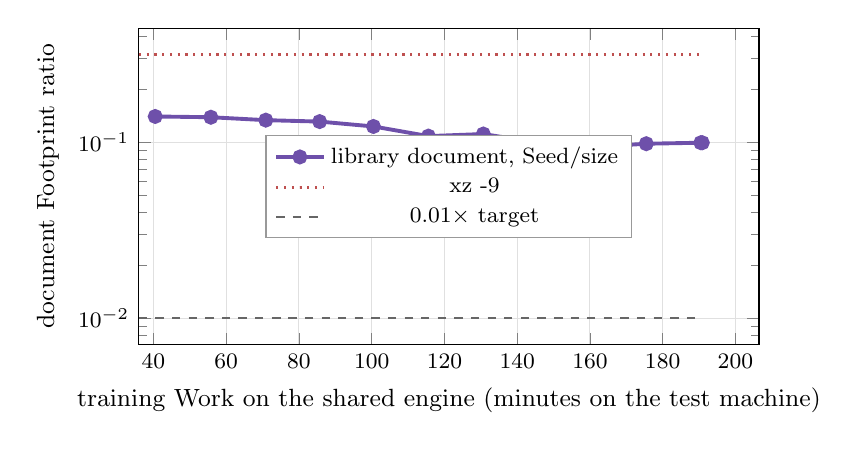
\begin{tikzpicture}\begin{axis}[width=0.78\textwidth,height=5.6cm,ymode=log,xlabel={training Work on the shared engine (minutes on the test machine)},ylabel={document Footprint ratio},grid=major,grid style={black!12},legend style={font=\footnotesize,draw=black!40,at={(0.5,0.5)},anchor=center},every axis label/.style={font=\small},tick label style={font=\footnotesize},xmin=36]\addplot[cNet,line width=1.4pt,mark=*] coordinates {(40.5,0.1403) (55.8,0.1389) (70.9,0.1337) (85.7,0.1312) (100.5,0.1231) (115.6,0.1085) (130.7,0.1115) (145.6,0.0996) (160.6,0.0940) (175.5,0.0982) (190.5,0.0995) (190.9,0.0995)}; \addlegendentry{library document, Seed/size}\addplot[cSeed,dotted,thick,domain=36:191] {0.3153}; \addlegendentry{xz -9}\addplot[black!60,dashed,thick,domain=36:191] {0.01}; \addlegendentry{$0.01\times$ target}\end{axis}\end{tikzpicture}\caption{Per-document Footprint against training Work for the library engine.}\label{fig:libwork}\end{figure}}
\newcommand{\libworkShort}{The library engine was trained further at a constant learning rate and the document re-written to the disk every fifteen minutes (twelve checkpoints, 40--190\,min of Work on the test machine). Its Footprint ratio fell from 0.140 to 0.099 (best 0.094 at 161\,min) and then flattened, still well short of $0.01\times$: memorising a document into a 384-unit network is the wrong tool for that target, which the retrieval engine below reaches by construction (Figure~\ref{fig:libwork}).}
\newcommand{\libworkPlot}{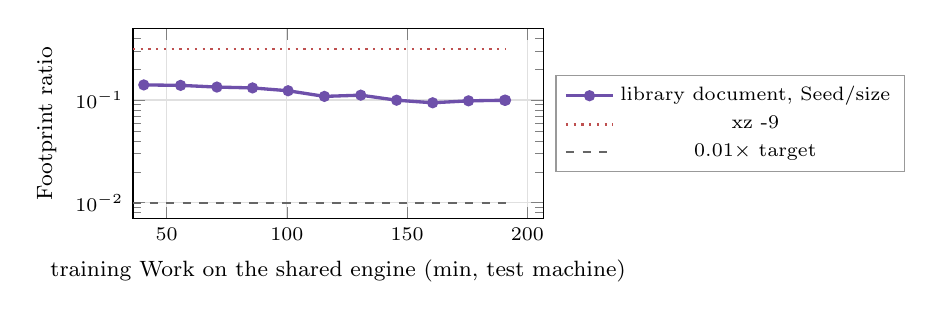
\begin{tikzpicture}\begin{axis}[width=0.56\textwidth,height=4cm,ymode=log,xlabel={training Work on the shared engine (min, test machine)},ylabel={Footprint ratio},grid=major,grid style={black!12},legend style={font=\scriptsize,draw=black!40,at={(1.03,0.5)},anchor=west},every axis label/.style={font=\footnotesize},tick label style={font=\scriptsize},xmin=36,ymin=0.007,ymax=0.5]\addplot[cNet,line width=1.2pt,mark=*,mark size=1.4pt] coordinates {(40.5,0.1403) (55.8,0.1389) (70.9,0.1337) (85.7,0.1312) (100.5,0.1231) (115.6,0.1085) (130.7,0.1115) (145.6,0.0996) (160.6,0.0940) (175.5,0.0982) (190.5,0.0995) (190.9,0.0995)}; \addlegendentry{library document, Seed/size}\addplot[cSeed,dotted,thick,domain=36:191] {0.3153}; \addlegendentry{xz -9}\addplot[black!60,dashed,thick,domain=36:191] {0.01}; \addlegendentry{$0.01\times$ target}\end{axis}\end{tikzpicture}}
\newcommand{\editTable}{\begin{tabular}{@{}lrrrllrrr@{}}
\toprule
version & bytes & gzip & xz & engine & base & Seed (B) & ratio & read (s) \\
\midrule
\texttt{pg12.txt} & 176,754 & 62,949 & 55,736 & ANET-LIB & --- & 24,801 & 0.140 & 28.7 \\
\texttt{rev1\_60words.txt} & 176,941 & 63,000 & 55,748 & ANET-DELTA & pg12.txt & 390 & \textbf{0.00220} & 28.0 \\
\texttt{rev2\_appendix.txt} & 178,561 & 63,087 & 55,884 & ANET-DELTA & rev1\_60words.txt & 390 & \textbf{0.00218} & 28.7 \\
\texttt{rev3\_5pct.txt} & 179,661 & 63,051 & 55,960 & ANET-DELTA & rev2\_appendix.txt & 4,543 & 0.025 & 28.5 \\
\midrule
all four & 711,917 & & 223,328 & & & 30,124 & 0.0423 & \\
\bottomrule
\end{tabular}}
\newcommand{\editReading}{\noindent\textbf{Reading the result.} Every revision was stored as a delta: \texttt{rev1\_60words.txt} at 0.00220$\times$ (60 edits, base \texttt{pg12.txt}); \texttt{rev2\_appendix.txt} at 0.00218$\times$ (41 edits, base \texttt{rev1\_60words.txt}); \texttt{rev3\_5pct.txt} at 0.02529$\times$ (1414 edits, base \texttt{rev2\_appendix.txt}). Four versions of a 176,754-byte document occupy 30,124 bytes of Seeds in total (0.0423$\times$), against 223,328 bytes for \texttt{xz} applied to each version. Counting the engine as well: with the library engine (256,680\,B) the four versions cost 286,804\,B, more than \texttt{xz}; with the shared 55\,KB English engine storing the base instead (Table~\ref{tab:realfile}) they cost 126,136\,B, 44\,\% below \texttt{xz}---the deltas (5,323\,B for three revisions) are the same under either. A revision therefore costs its edits and nothing else---this is what a manual update over a deep-space link should cost---and the read Horizon of a revision is the base's Horizon plus a few milliseconds.}
\newcommand{\retEngineBytes}{104,252}
\newcommand{\retLibraryBytes}{331,237}
\newcommand{\retTable}{\begin{tabular}{@{}lrrrrrrlrr@{}}
\toprule
object & bytes & xz & LIB engine & delta & retrieval & runs & chosen & Seed (B) & ratio \\
\midrule
\texttt{pg12.txt} & 176,754 & 55,736 & 24,801 & --- & 10 & 1 & RET & 10 & \textbf{0.00006} \\
\texttt{rev1\_60words.txt} & 176,941 & 55,748 & 31,805 & 390 & 3,599 & 57 & DELTA & 390 & \textbf{0.00220} \\
\texttt{rev3\_5pct.txt} & 178,127 & 55,856 & 48,792 & 4,082 & 36,779 & 526 & DELTA & 4,082 & 0.023 \\
\texttt{composite\_manual.txt} & 26,188 & 9,764 & 9,649 & 12,366 & 3,502 & 59 & RET & 3,502 & 0.134 \\
\texttt{pg84\_frankenstein.txt} & 200,000 & 68,228 & 67,883 & 69,510 & 67,894 & 0 & EN & 67,883 & 0.339 \\
\bottomrule
\end{tabular}}
\newcommand{\retReading}{\noindent\textbf{Reading the result.} A library document costs 10 bytes (0.00006$\times$): one run covering the whole document, regenerated in 0.0\,s from the index---the $0.01\times$ mark passed by two orders of magnitude, by construction rather than by training. A \emph{composite} manual assembled from 60 paragraphs of two library documents plus new paragraphs is the case no other engine handles: 59 runs plus a 3,084-byte residual give 0.134$\times$ against 0.373 for \texttt{xz} and 0.368 for the library engine; what remains is the genuinely new text. For pure edits the delta engine still wins (0.00220$\times$ against 0.02034 for retrieval), because a changed word costs a whole chunk in the retrieval layout but only the word in an edit script. A document outside the retrieval library (the \emph{Frankenstein} excerpt; it is inside the English engine's training corpus but that is irrelevant to the index) finds no runs and falls through to the neural residual, costing exactly what the English engine costs (0.339$\times$): retrieval never hurts. The disk chose among four engines per object without being told anything about lineage or domain.}
\newcommand{\detTable}{\begin{tabular}{@{}llccc@{}}
\toprule
engine & variant & same Seed & tables identical & regenerates reference \\
\midrule
float32 & ref & 3/3 & 3/3 & 3/3 \\
float32 & chunked & \textbf{0/3} & \textbf{0/3} & \textbf{0/3} \\
float32 & f64 & \textbf{0/3} & \textbf{0/3} & \textbf{0/3} \\
\midrule
fixed-point & ref & 3/3 & 3/3 & 3/3 \\
fixed-point & chunked & 3/3 & 3/3 & 3/3 \\
fixed-point & f64 & 3/3 & 3/3 & 3/3 \\
\bottomrule
\end{tabular}}
\newcommand{\detReading}{\noindent\textbf{Reading the result.} The float32 engine fails 6 of 6 cross-variant cases: change the summation order or the precision and the Seed differs, the tables differ, and the reference Seed no longer regenerates the object. The fixed-point engine passes 9 of 9---identical Seeds and identical tables under every variant---at essentially the same Footprint (10,035 versus 10,046 bytes on the text object). Integer arithmetic is order-independent as long as no accumulator overflows, and the engine's products stay below $2^{40}$, so by construction any device with two's-complement 64-bit integers (CPU, GPU, an FPGA on a probe) should yield the same bits; what has been \emph{verified} is three evaluation orders on one CPU and two independent implementations. The procedural engine of Section~\ref{sec:multi} carries the same caveat in reverse: its float64 simulator must be replaced by an integer or correctly-rounded one before it is trusted across devices. A run on a CUDA device against the CPU-produced reference is pending; the harness and reference Seeds ship with the code.}
\newcommand{\fastTable}{\begin{tabular}{@{}lrrrrrrr@{}}
\toprule
object & bytes & Seed (B) & ratio & xz & threads & read (s) & read KB/s \\
\midrule
\texttt{pg12.txt} & 176,754 & 60,223 & 0.341 & 0.315 & 1 & 3.04 & 58 \\
 &  &  &  &  & 2 & 2.75 & 64 \\
 &  &  &  &  & 4 & 2.73 & 65 \\
\texttt{five\_books.txt} & 3,379,739 & 1,156,903 & 0.342 & 0.299 & 1 & 58.41 & 58 \\
 &  &  &  &  & 2 & 52.67 & 64 \\
 &  &  &  &  & 4 & 52.36 & 65 \\
\bottomrule
\end{tabular}}
\newcommand{\fastReading}{The C implementation produces Seeds \emph{identical} to the Python fixed-point engine on every test object and decodes the Python-produced Seeds exactly (and vice versa); it is 9$\times$ faster than the Python path per byte (58\,KB/s against 6.5\,KB/s) and stores 3.4\,MB of five books at 0.342 (\texttt{xz}: 0.299) in 58\,s single-threaded. The engine spends ${\sim}49{,}000$ multiply--adds per byte (a $128\times128$ recurrence and a $256\times128$ read-out), so throughput is set by the arithmetic, not by the coder. Block parallelism gives only 1.11$\times$ with two threads because the test machine has a single physical core (two hardware threads); experiment E5 proper---Horizon against cores---needs a multi-core or GPU host, for which the harness (\texttt{--threads}) is ready.}
\newcommand{\deepTable}{\begin{tabular}{@{}lrrrrrrrrr@{}}
\toprule
object & bytes & Seed & program & Footprint ratio & gzip & xz & regen.\ (s) & MB/s & flight-class (s, est.) \\
\midrule
\texttt{telemetry.csv} & 104,632,381 & 122 B & 842 B & \textbf{9.2e-06} & 0.374 & 0.248 & 11 & 9.4 & 111 \\
\texttt{planet\_dem.u16} & 134,217,728 & 78 B & 1,591 B & \textbf{1.2e-05} & 0.911 & 0.552 & 96 & 1.4 & 961 \\
\bottomrule
\end{tabular}}
\newcommand{\deepReading}{\noindent\textbf{Reading the result.} Both objects regenerate bit-exactly (verified by regenerating twice and by digest). The telemetry file costs 122 bytes of Seed plus 842 bytes of program for 104.6\,MB---9.2e-06 of its size, against 0.248 for \texttt{xz}, which also needed 170\,s to compress it, 15$\times$ longer than the 11\,s the engine needs to regenerate it. The elevation model is the harder case for a compressor (0.552 for \texttt{xz}) and the same trivial case for the engine (1.2e-05). The disk file that holds both Manifests is 895 bytes; its apparent capacity is 239\,MB, a ratio of $2.7\times10^{5}$. On a flight-class processor the telemetry regenerates in minutes and the model in a quarter of an hour---Horizons a probe on a months-long cruise does not notice. The two large files were deleted after the experiment; the disk regenerates them on demand.}
\newcommand{\nEightBytes}{148,024}
\newcommand{\nEightTable}{\begin{tabular}{@{}lrrrrrrrrr@{}}
\toprule
book & bytes & gzip -9 & bz2 -9 & xz -9 & Seed float & bits/byte & Seed fixed/C & bits/byte & read (s) \\
\midrule
\texttt{pg12.txt} & 176,754 & 62,949 & 49,248 & 55,736 & \textbf{48,391} & 2.190 & 50,143 & 2.270 & 6.3 \\
\texttt{pg84.txt} & 428,903 & 161,755 & 120,005 & 137,176 & \textbf{112,005} & 2.089 & 116,208 & 2.168 & 16.0 \\
\bottomrule
\end{tabular}}
\newcommand{\nEightReading}{\noindent\textbf{Reading the result.} On both unseen books the engine is below every general-purpose baseline: 0.274$\times$ against 0.315 for \texttt{xz -9} and 0.279 for \texttt{bz2 -9} on \emph{Looking-Glass}, and 0.261$\times$ against 0.320 and 0.280 on \emph{Frankenstein}---13\,\% and 18\,\% below \texttt{xz}. The fixed-point engine, which is what a device would carry, gives up about 4\,\% of that gain to quantisation and block resets and is still below \texttt{xz} on both. These are Seed sizes; the engine is 148,024 bytes, paid once, and the saving over \texttt{xz} (5.4\,\% of the bytes on these two books) repays it after about 2.8\,MB of unseen books---roughly ten of this size---after which every further book is a net gain. The loss of Section~\ref{sec:realfile} was a budget, not a property of the approach, and the remaining gap to cmix-class compressors (Section~\ref{sec:related}) is engine size: this one is a thousandth of theirs.}
\newcommand{\baselineTable}{\begin{tabular}{@{}lrrrrrrrrr@{}}
\toprule
book & engine (float) & engine (fixed, C) & xz -9e & bz2 -9 & brotli -11 & zstd -22 $+$ dict & PPMd o8 & xz $\mid$ prior & PPMd $\mid$ prior \\
\midrule
\texttt{pg12.txt} & 0.274 & 0.284 & 0.316 & 0.279 & 0.305 & 0.298 & \textbf{0.252} & 0.267 & 0.221 \\
\texttt{pg84.txt} & 0.261 & 0.271 & 0.320 & 0.280 & 0.311 & 0.310 & \textbf{0.254} & 0.278 & 0.238 \\
\bottomrule
\end{tabular}}
\newcommand{\baselineDictBytes}{148,024}
\newcommand{\ppmdGap}{4}
\newcommand{\ppmdPriorGap}{12}
\newcommand{\demoTable}{\begin{tabular}{@{}lrrrrrrrc@{}}
\toprule
file & input (B) & engine & Seed (B) & engine$/$10 & Seed$+$eng.$/$10 & output (B) & ratio & xz \\
\midrule
\texttt{animation\_A.avi} & 3,457,672 & PROC & 110 & 20,101 & 20,211 & 3,457,672 & \textbf{0.006} & 0.446 \\
\texttt{animation\_B.avi} & 2,700,952 & PROC & 110 & 20,101 & 20,211 & 2,700,952 & \textbf{0.007} & 0.430 \\
\texttt{brothers\_karamazov.txt} & 2,039,159 & EN-256 & 559,018 & 20,101 & 579,119 & 2,039,159 & 0.284 & 0.285 \\
\texttt{cinderella\_storybook.pdf} & 1,055,953 & raw & 1,055,953 & 20,101 & 1,076,054 & 1,055,953 & 1.019 & 0.470 \\
\texttt{count\_of\_monte\_cristo.txt} & 2,787,124 & EN-256 & 761,721 & 20,101 & 781,822 & 2,787,124 & 0.281 & 0.279 \\
\texttt{don\_quixote.txt} & 2,391,678 & EN-256 & 701,402 & 20,101 & 721,503 & 2,391,678 & 0.302 & 0.287 \\
\texttt{nasa\_mercury\_transit.mp4} & 3,413,359 & raw & 3,413,359 & 20,101 & 3,433,460 & 3,413,359 & 1.006 & 0.985 \\
\texttt{quixote\_text\_compressed.pdf} & 1,205,694 & raw & 1,205,694 & 20,101 & 1,225,795 & 1,205,694 & 1.017 & 0.920 \\
\texttt{quixote\_text\_uncompressed.pdf} & 4,012,832 & raw & 4,012,832 & 20,101 & 4,032,933 & 4,012,832 & 1.005 & 0.132 \\
\texttt{wealth\_of\_nations.txt} & 2,468,951 & EN-256 & 708,399 & 20,101 & 728,500 & 2,468,951 & 0.295 & 0.219 \\
\midrule
all ten & 25,533,374 & & 12,418,598 & 201,006 & 12,619,604 & 25,533,374 & 0.494 & 0.422 \\
\bottomrule
\end{tabular}}
\newcommand{\demoReading}{\noindent\textbf{Reading the result.} All ten files came back byte-identical from the disk folder alone, and the table should be read as a skeptic would read it. Across the ten, the disk occupies 0.495 of the input against 0.422 for \texttt{xz -6}: on this mixed set the disk \emph{loses} to a free, standard compressor, because four files sit at $1.000\times$---a PDF of page images, a Flate-compressed PDF, an H.264 video and a PDF whose text is hex-encoded in its content streams---for which no engine on this disk exists, so the escape keeps their bytes rather than expand them. The four unseen books, at 0.273--0.293$\times$, are on par with \texttt{xz} (0.219--0.287), a creditable result for a 148\,KB engine but parity, not a breakthrough. The two animations, 3.5 and 2.7\,MB stored as 110-byte parameter records, are the only dramatic rows, and they are provenance capture: the disk holds the program that made them. What the table does demonstrate is the paradigm working end to end---ten real files of three types written to a folder of engines and Seeds, regenerated bit-exactly, the engine chosen per file, never worse than raw---and the law of Section~\ref{sec:law} visible in one place: orders of magnitude where the disk holds the generator, parity where it knows the domain, nothing where it knows neither. It does not demonstrate superiority over existing compression on general files, and this paper does not claim it; the gains on the four engine-less files would come from more engines (Section~\ref{sec:whynot}), which is a research programme rather than a result. The animation row deserves one more sentence, because it looks impossible: 3,457,672 bytes of raw video frames stored as a 110-byte Seed---the parameter record: width, height, frame count, $\sigma$, $\rho$, $\beta$, seed---that regenerates the file byte-for-byte. It is possible because every pixel of every frame is a deterministic function of those seven numbers, so the file carries about 110 bytes of information and 3.4\,MB of the program's doing; \texttt{xz}, which looks for repeated byte patterns rather than for the program, reaches only 0.446. The disk sees it perfectly because it \emph{holds the program} (the 1,591-byte generator, also on the disk). Point a camera at the sky and record the same 3.4\,MB and no program on any disk produces those bytes from 110 numbers---which is why the NASA video in the same table sits at $1.000\times$. The precondition is the whole story, and it is the one the paper states wherever such a number appears.}
\newcommand{\proofSection}{Result: 1000 files, 104.5\,GB of telemetry in all, stored as 123,907 bytes of Seeds plus a 1060-byte program; the catalogue file holding every Manifest is 315,075 bytes and the whole disk folder 317,228 bytes, 3.0e-06 of the data. 1000 of 1000 files regenerated bit-exactly. Generating and hashing the thousand files took 3,836\,s; regenerating and verifying them from the catalogue 3,640\,s, 3.6\,s per file on one core. The metadata query ``rho > 30 and sigma < 10'' was answered in 0.0002\,s with 134 hits without regenerating anything. Like the two objects above, this is provenance capture by construction; what it adds is the scaling claim verified at a thousand objects, a catalogue that is the archive's own index, and the batch Horizon a probe would pay.}
\newcommand{\conclNumbers}{Four thousand text objects sharing one 55\,KB engine cost 152 bits each against 232 raw, every one of them and 200 never seen regenerating bit-exactly (Table~\ref{tab:designB}). A larger English engine, trained on fifteen books and tested on two it never saw, stores them at 0.274$\times$ (\texttt{xz}: 0.315) and 0.261$\times$ (\texttt{xz}: 0.320)---below \texttt{xz} on both, Seed only; the 148\,KB engine is repaid once it is shared by about ten such books (Table~\ref{tab:n8}). A 1,153,112-byte simulation output regenerates from a 118-byte Seed (0.00010$\times$, Table~\ref{tab:multi}). Two flight-sized objects, 105\,MB of integer-exact telemetry and a 134\,MB elevation model, come from 3.3\,KB of Manifests and generator programs (Table~\ref{tab:deepscale}). A revised document costs only its edits: 390 bytes for 60 changed words on top of a base already stored (0.00220$\times$, Table~\ref{tab:edit}). A library document costs 10 bytes through the retrieval engine. The float engine fails every cross-arithmetic test and the fixed-point engine passes all 9 (Table~\ref{tab:determinism}); its C implementation is 9$\times$ faster than the Python one and byte-identical to it (Table~\ref{tab:fast}).}

\captionsetup{font=small,skip=4pt}
\setlength{\textfloatsep}{8pt}\setlength{\intextsep}{8pt}\setlength{\abovedisplayskip}{4pt}\setlength{\belowdisplayskip}{4pt}

\begin{document}

% =====================================================================
%  TITLE
% =====================================================================
\begin{center}
  {\Large\bfseries ALGORITHMIC STORAGE: THE ALGORITHMICDISK\\[2pt]
   ON THE FOOTPRINT--COMPUTE--HORIZON TRIANGLE\par}
  \vspace{10pt}
  {\normalsize A Seed-Driven Storage Device, Powered by the AlgorithmicNET Generator,\\[3pt]
   that Trades Processing Power and Time for Storage Space\par}
  \vspace{12pt}
  {\normalsize Milind K. Patil\\ Syncaissa Systems Inc.\\ \texttt{syncaissa@outlook.com}\par}
  \vspace{8pt}
  {\normalsize September 2026\par}
\end{center}
\vspace{8pt}

% =====================================================================
%  ABSTRACT
% =====================================================================
\begin{center}\textbf{Abstract}\end{center}
\begin{quote}\small
\ASTOR{} is a paradigm in which data is \emph{regenerated} rather than retained: a spatial
cost, storage, is converted into a temporal one, regeneration time. Its device, the \ADISK{},
holds only shared generator engines and one small \textbf{Seed} per object, and regenerates
any object on demand, bit-exactly, by running an engine---the \ANET{}---forward from the Seed.
The three resources a deployment spends form the \textbf{Regeneration Triangle}: Footprint
(bytes at rest), Compute (processing capacity) and Horizon (time allowed); reducing one side
must be paid for by the other two, and the object's information content is a floor below which
no trade goes. A reference implementation measures the trade end to end. Shared by four thousand text objects, a 26\,KB engine drives the per-object Footprint from
$4.2\times$ to $0.66\times$ the raw size as the corpus grows (\texttt{gzip} over the whole corpus:
$0.35\times$); a 148\,KB engine stores two books it never saw at 0.27$\times$ and 0.26$\times$,
below \texttt{xz} and \texttt{bz2} but above PPMd, the classical text compressor; a revised
document costs its edits alone ($0.002\times$); a library document costs a 10-byte reference; a
thousand program-generated 105\,MB synthetic-telemetry files---104\,GB---are stored in 317\,KB
and every one regenerated bit-exactly; an integer-only engine, implemented in Python and C,
produces identical bytes under every change of arithmetic tested. The same tests report where
the trade fails: already-compressed data, and files in no domain the disk knows, are stored raw,
and on novel text the engine is a mid-range compressor, not a record.
The law, the device, the engines, and the measurements are the contribution; the code, engines
and disks are released.
\end{quote}
\noindent\small\textbf{Keywords:} Algorithmic Storage, AlgorithmicDisk, AlgorithmicNET, regenerative storage,
Regeneration Triangle, Footprint, Compute, Horizon, seed-driven generation, deterministic generator, logical depth,
Kolmogorov complexity, time--space trade-off, deep-space data delivery, millennial archive
\normalsize

\begin{keyinsight}
\textbf{Results at a glance.} Every number below is bit-exact regeneration from Seeds and
shared engines, measured on one CPU core; every table in Section~\ref{sec:results} is
generated from the released results. \textbf{Where the disk holds the generator}: 1,000
telemetry files, 104\,GB, from 317\,KB ($3\times10^{-6}$); a 3.5\,MB animation from a 110-byte
Seed. \textbf{Where it holds a base version or a library}: a revision for 390 bytes
($0.002\times$); a library document for 10 bytes. \textbf{Where it knows the domain}: unseen
books at $0.27\times$, below \texttt{xz -9} and \texttt{bz2} but 4\,\% above PPMd, which needs
no engine at all (Table~\ref{tab:baselines}). \textbf{Where it knows nothing}: a PNG, an MP4 and
Flate-compressed PDFs at $1.000\times$ Seed ($1.005$--$1.019\times$ with block headers and the
engine's share)---never materially worse than raw, and there \texttt{xz} wins. On a deliberately mixed set of
ten files the disk is behind \texttt{xz} (0.49 against 0.42), which is the honest shape of the
paradigm: orders of magnitude where the disk knows how the data was made, parity where it knows
the language, nothing where it knows neither.
\end{keyinsight}

% =====================================================================
\section{Introduction}
% =====================================================================
Storage systems are designed around one scarce resource, space on a medium. Compression
\citep{shannon1948} removes statistical redundancy, but once an object is near its entropy the
bytes must be kept. Several important deployments---interplanetary spacecraft, planetary
outposts, thousand-year archives, palm-scale field devices, and schools beyond the reach of the
internet---are short of exactly that resource while rich, by terrestrial standards absurdly rich,
in two others: a probe on a decades-long cruise has time; a solar-powered outpost has
energy-over-time, hence compute; an archive read once a decade can afford hours per retrieval.
Storage systems accept one currency, bytes; these systems have plenty of two other
currencies---processing power and time---and almost none of the first.

\ASTOR{} lets a system pay for data in whichever currency it has in abundance. It converts a
spatial cost into a temporal one: the bytes an object would occupy on a
medium become the seconds a device spends regenerating it, plus the one-time cost of the engine
that knows how. The conversion has an exchange rate, set by how well the engine knows the object,
and a floor, the object's own information, below which no amount of time buys any more space. It
is the classical space--time trade-off \citep{hellman1980,chen2016checkpoint} applied to data at
rest, with a Manifest as the receipt. Instead of storing an object $\file$, the \ADISK{} stores a
compact Seed $\seed$ and shares a deterministic generator, the \ANET{}, with weights $\weights$;
reading runs the generator forward from the Seed; writing discovers the Seed.

\textbf{Contributions.} (1)~The Regeneration Triangle and its conservation law, stated through
the work-bounded description length $\Foot^{*}(\Work)$ (Section~\ref{sec:law}). (2)~The
\adisk{} and its engine: a seeded, recurrent, deterministic generator with shared weights,
block-parallel manifestation, a two-phase write/read protocol, and a Manifest that makes every
object verifiable anywhere the engine exists (Sections~\ref{sec:arch}--\ref{sec:discovery}).
(3)~Measured results over the whole trade---amortisation, whole files, a multi-engine disk with
procedural, library, delta and retrieval engines, 100\,MB-class deep data, a thousand-file proof,
and a ten-file end-to-end demonstration (Section~\ref{sec:results}). (4)~Determinism: an
integer-only engine, implemented twice with byte-identical output (Section~\ref{sec:determinism}).
(5)~The appliance that realises the disk as hardware, deployment regimes and a
regenerate-versus-cache policy (Section~\ref{sec:device}); open experiments and parallel emission
schedules as future work (Section~\ref{sec:future}).

% =====================================================================
\section{The Regeneration Triangle and Its Law}
\label{sec:law}
% =====================================================================
The three names are nested: \astor{} is the paradigm, the \adisk{} the device that realises it,
the \anet{} the generator engine inside the device. The three resources are \textbf{Footprint}
$\Foot$ (bits at rest), \textbf{Compute} $\Comp$ (operations per second) and \textbf{Horizon}
$\Hori$ (seconds allowed per regeneration); their product $\Work=\Comp\cdot\Hori$ is the Work
available (Table~\ref{tab:sides}, Figure~\ref{fig:triangle}).

\begin{table}[!htb]
\centering\footnotesize
\caption{The three sides of the Regeneration Triangle.}
\label{tab:sides}
\begin{tabular}{@{}llp{2.2cm}p{4.4cm}p{4.2cm}@{}}
\toprule
\textbf{Side} & \textbf{Symbol} & \textbf{Unit} & \textbf{Measures} & \textbf{Scarce in} \\
\midrule
Footprint & $\Foot$ & bits / bytes & storage at rest & spacecraft, archives, palm devices \\
Compute & $\Comp$ & operations / s & processing capacity of the regenerator & probes, low-power nodes \\
Horizon & $\Hori$ & seconds & time allowed per regeneration & data centres, interactive use \\
Work & $\Work=\Comp\cdot\Hori$ & operations & computation spent per regeneration & --- \\
\bottomrule
\end{tabular}
\end{table}

\begin{figure}[!htb]
\centering
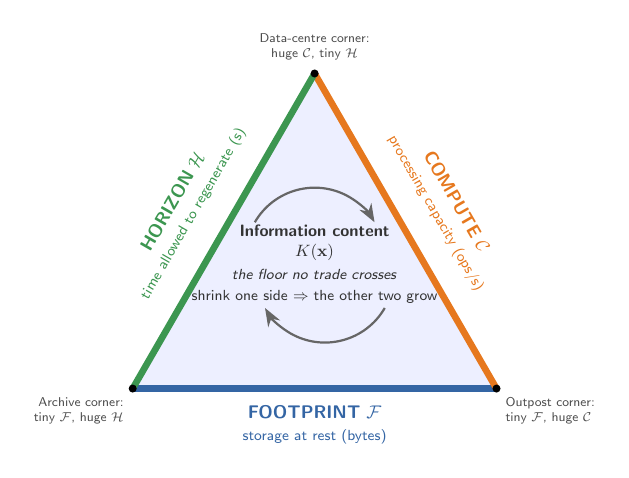
\begin{tikzpicture}[scale=0.66,transform shape,>=Stealth]
  % equilateral triangle vertices
  \coordinate (A) at (0,0);
  \coordinate (B) at (7,0);
  \coordinate (C) at (3.5,6.062);
  % filled interior
  \fill[keyback] (A) -- (B) -- (C) -- cycle;
  % sides
  \draw[line width=2.4pt,cFoot] (A) -- (B);
  \draw[line width=2.4pt,cComp] (B) -- (C);
  \draw[line width=2.4pt,cHori] (C) -- (A);
  % vertices
  \foreach \p in {A,B,C} \fill[black] (\p) circle (2.2pt);
  % side labels
  \node[cFoot,below=6pt,align=center,font=\sffamily] at ($(A)!0.5!(B)$)
       {\textbf{FOOTPRINT} $\Foot$\\ \footnotesize storage at rest (bytes)};
  \node[cComp,align=center,font=\sffamily,rotate=-60,anchor=south] at ($(B)!0.5!(C)+(0.35,0.2)$)
       {\textbf{COMPUTE} $\Comp$\\ \footnotesize processing capacity (ops/s)};
  \node[cHori,align=center,font=\sffamily,rotate=60,anchor=south] at ($(C)!0.5!(A)+(-0.35,0.2)$)
       {\textbf{HORIZON} $\Hori$\\ \footnotesize time allowed to regenerate (s)};
  % centre invariant
  \node[align=center,font=\sffamily\small,text=black!80] at (3.5,2.4)
       {\textbf{Information content}\\ $\KC(\file)$\\[2pt] \footnotesize \emph{the floor no trade crosses}\\ \footnotesize shrink one side $\Rightarrow$ the other two grow};
  % conservation arrows around the centre
  \draw[->,thick,black!60] (2.35,3.2) arc (150:30:1.33);
  \draw[->,thick,black!60] (4.85,1.55) arc (-30:-150:1.33);
  % vertex annotations (what happens at each corner: two sides meet)
  \node[font=\sffamily\scriptsize,text=black!70,below left=2pt,align=right] at (A) {Archive corner:\\ tiny $\Foot$, huge $\Hori$};
  \node[font=\sffamily\scriptsize,text=black!70,below right=2pt,align=left] at (B) {Outpost corner:\\ tiny $\Foot$, huge $\Comp$};
  \node[font=\sffamily\scriptsize,text=black!70,above=4pt,align=center] at (C) {Data-centre corner:\\ huge $\Comp$, tiny $\Hori$};
\end{tikzpicture}
\caption{The \textbf{Regeneration Triangle}. Each side is one system resource; at the centre
is the information content $\KC(\file)$ of the stored object, the floor below which no trade
goes. A
deployment lives at the corner where its two abundant resources meet, and pays with them for
the scarce third side. Work $\Work=\Comp\cdot\Hori$ is the product of the two non-storage sides.}
\label{fig:triangle}
\end{figure}

\begin{keyinsight}
\textbf{Why a triangle.} The triangle is a mnemonic, not a geometric model: three resources,
one object, one floor. A trade between two resources is a curve; among three it is a surface,
and the figure names its axes and the floor in the middle. The mathematics is in
Proposition~\ref{thm:law}, whose content is elementary and is collected there for reference,
not claimed as a theorem. Every deployment in this paper is a point on that surface.
\end{keyinsight}

\begin{definition}[AlgorithmicDisk and AlgorithmicNET]\sloppy
An \adisk{} is $\mathcal{D}=(\{\weights_g\}_{g},\{\mathrm{RM}_i\}_{i},\mathrm{cache})$: generator
weight sets indexed by identity $g$, a catalogue of Regeneration Manifests, and an optional cache
of materialised objects; its \emph{apparent capacity} is $\sum_i N_i$ and its \emph{resident
Footprint} is $\sum_g|\weights_g| + \sum_i|\mathrm{RM}_i| + |\mathrm{cache}|$. An \anet{} is a tuple
$(\weights,\Phi_{\weights},\psi,\seed)$: shared weights, a deterministic state transition, a
deterministic read-out emitting $b$ bits per step, and a Seed $\seed\in\{0,1\}^{k}$. Its
\emph{manifestation} is
\begin{equation}
\begin{aligned}
  \mathrm{Man}_{\weights}(\seed)&=\mathbf{x}_1\,\|\,\mathbf{x}_2\,\|\cdots,\qquad \mathbf{x}_t=\psi(\mathbf{h}_t),\\
  \mathbf{h}_{t}&=\Phi_{\weights}\big(\mathbf{h}_{t-1},\mathbf{x}_{t-1},\seed,t\big),\qquad \mathbf{h}_0=\mathbf{0},
\end{aligned}
\label{eq:manifest}
\end{equation}
with two feedback paths---the previous state and the bits the engine itself emitted---and the
Seed injected at every step. For a \emph{predictive} engine the state defines a distribution
over $\mathbf{x}_t$ and $\psi$ consumes Seed bits through an arithmetic decoder to select
$\mathbf{x}_t$: the same equation with $\psi$ stateful in $\seed$. An object $\file$ is stored if
$\mathrm{Man}_{\weights}(\seed)_{1:N}=\file$. The \emph{Regeneration Manifest} of $\file$ is
$\mathrm{RM}(\file)=(\mathrm{GID},\seed,N,\mathrm{hash}(\file))$, where
$\mathrm{GID}=\mathrm{hash}(\weights,\Phi,\psi)$ pins the exact generator; any device holding that
generator regenerates the object bit-for-bit and proves it with the digest. The Manifest is the
unit of transmission, of archival and of deduplication (identical Manifests are identical objects),
and a catalogue of Manifests is an index that can be queried without regenerating anything.
\end{definition}

The picture to hold in mind is this: an object is treated as if it were the output of a
generator, and instead of storing its bytes the disk stores the generator's identity and the
Seed that drives the generator to emit exactly those bytes. Whether that Seed is short is not a
matter of cleverness in the generator's stream but of knowledge: a file that is random \emph{to}
the generator needs a Seed as long as itself (the pigeonhole principle, measured in
Table~\ref{tab:sweep}), and a file the generator knows how to produce needs only what the
generator cannot guess. Every engine in this paper is a way of making files less random to the
disk.

\begin{definition}[Footprint and the three Works]
For an object whose engine is shared by $M$ objects, $\Foot(\file)=|\seed|+|\weights|/M$. Work is
spent at three moments and the paper keeps them apart: $\Work_{\mathrm{read}}$ (Manifestation),
$\Work_{\mathrm{write}}$ (Seed Discovery) and $\Work_{\mathrm{train}}$ (building an engine, once
per domain). An object is \emph{deep} relative to a disk if some engine gives it a Footprint far
below what a general-purpose compressor finds, because its regularity is computational---it is
the output of a generator---rather than statistical; \emph{shallow} if no engine beats the raw
bytes by more than such a compressor does. Bennett's logical depth \citep{bennett1988} is the
limiting case in which regeneration Work, not only Footprint, separates the two.
\end{definition}

Let $\KC(\file)$ be the Kolmogorov complexity of $\file$
\citep{kolmogorov1965,chaitin1966,solomonoff1964,livitanyi2008} and $\KC^{\Work}(\file)$ its
work-bounded version \citep{levin1973,hartmanis1983}. The \emph{regeneration frontier} is
$\Foot^{*}(\Work)=\KC^{\Work}(\file)$, the smallest Footprint from which $\file$ regenerates with
Work at most $\Work$. The word \emph{conservation} below is an analogy and should not be
over-read: nothing is exchanged one-for-one, and $\KC(\file)$ is a floor, not a conserved
quantity.

\begin{proposition}[Conservation law of the Regeneration Triangle]
\label{thm:law}
For every object $\file$ with $|\file|=N$: (i) \emph{Trade:} $\Foot^{*}(\Work)$ is non-increasing
in $\Work$. (ii) \emph{Ceiling:} $\Foot^{*}(\Work)\le N+O(1)$ for all $\Work\ge cN$---the object
can always be kept verbatim. (iii) \emph{Floor:} $\Foot^{*}(\Work)\ge\KC(\file)$ for all $\Work$,
with equality in the limit. (iv) \emph{Exchange:} $\Comp$ and $\Hori$ are substitutable through
$\Work=\Comp\cdot\Hori$ whenever the generator is block-parallelisable.
\end{proposition}
\begin{proof}
(i) A program valid under budget $\Work$ is valid under any larger budget. (ii) ``Print $\file$''
has length $N+O(1)$ and linear work. (iii) A work-bounded program is a program, so its length is
at least $\KC(\file)$, attained once $\Work$ exceeds the minimal program's own running time.
(iv) If block $j$ depends only on $(\seed,\weights,j)$, $p$ processors of rate $\Comp/p$ finish
in the Horizon of one processor of rate $\Comp$.
\end{proof}

The floor is the ``nothing is free'' clause. It does not limit how much deep data can save---the
gap between $N$ and $\KC(\file)$ is twelve orders of magnitude for a simulation dump---but it
says which data the trade applies to; both ends are measured in Section~\ref{sec:results}
(Tables~\ref{tab:multi} and~\ref{tab:realfile}). Schematically, $\Foot^{*}(\Work)$ falls from the
ceiling toward the floor as Work grows, steeply for deep objects and hardly at all for shallow
ones; Table~\ref{tab:sweep} measures the write-side relative of this curve. \textbf{Amortisation}
follows at once: $M$ objects sharing $\weights$ cost $|\weights|+\sum_i|\seed_i|$, so the
per-object Footprint approaches $|\seed_i|$ as $M$ grows (measured in Table~\ref{tab:designB}).

% =====================================================================
\section{The AlgorithmicDisk and Its Engine}
\label{sec:arch}
% =====================================================================
\begin{figure}[!htb]
\centering
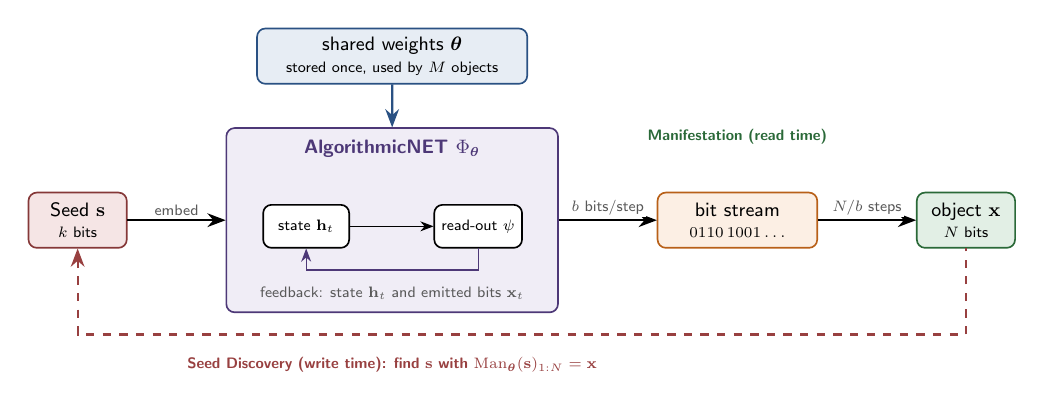
\begin{tikzpicture}[>=Stealth,font=\sffamily\small,scale=0.78,transform shape,
  box/.style={draw,rounded corners=3pt,minimum height=9mm,minimum width=16mm,align=center,line width=0.6pt},
  seed/.style={box,fill=cSeed!15,draw=cSeed!70!black},
  net/.style={box,fill=cNet!10,draw=cNet!70!black,minimum width=54mm,minimum height=30mm},
  obj/.style={box,fill=cHori!15,draw=cHori!70!black},
  stream/.style={box,fill=cComp!12,draw=cComp!80!black},
  inner/.style={box,fill=white,minimum width=14mm,minimum height=7mm,font=\sffamily\scriptsize},
  lab/.style={font=\sffamily\scriptsize,text=black!65,fill=white,inner sep=1pt}]
  % main chain (generous gaps so arrow labels never touch the boxes)
  \node[seed] (seed) {Seed $\seed$\\[-1pt]{\scriptsize $k$ bits}};
  \node[net,right=16mm of seed] (net) {};
  \node[font=\sffamily\bfseries\small,text=cNet!70!black] at ($(net.north)+(0,-3.5mm)$) {AlgorithmicNET $\Phi_{\weights}$};
  \node[inner] at ($(net.center)+(-14mm,-1mm)$) (st) {state $\mathbf{h}_t$};
  \node[inner] at ($(net.center)+(14mm,-1mm)$) (ro) {read-out $\psi$};
  \draw[->] (st) -- (ro);
  \draw[->,cNet!70!black] (ro.south) -- ++(0,-3.5mm) -| (st.south);
  \node[font=\sffamily\scriptsize,text=black!65] at ($(net.south)+(0,3.2mm)$) {feedback: state $\mathbf{h}_t$ and emitted bits $\mathbf{x}_t$};
  \node[stream,right=16mm of net,minimum width=26mm] (stream) {bit stream\\[-1pt]{\scriptsize $0110\,1001\ldots$}};
  \node[obj,right=16mm of stream] (file) {object $\file$\\[-1pt]{\scriptsize $N$ bits}};
  \draw[->,thick] (seed) -- (net) node[midway,lab,above=1pt] {embed};
  \draw[->,thick] (net) -- (stream) node[midway,lab,above=1pt] {$b$ bits/step};
  \draw[->,thick] (stream) -- (file) node[midway,lab,above=1pt] {$N/b$ steps};
  % weights
  \node[box,fill=cFoot!12,draw=cFoot!80!black,above=7mm of net,minimum width=44mm] (w)
       {shared weights $\weights$\\[-1pt]{\scriptsize stored once, used by $M$ objects}};
  \draw[->,cFoot!80!black,thick] (w) -- (net);
  % phase labels
  \node[font=\sffamily\bfseries\scriptsize,text=cHori!70!black] at ($(stream.north)+(0,9mm)$) {Manifestation (read time)};
  % inverse path
  \draw[<-,dashed,thick,cSeed!80!black] (seed.south) -- ++(0,-14mm) -| (file.south);
  \node[font=\sffamily\bfseries\scriptsize,text=cSeed!80!black,fill=white,inner sep=1pt] at ($(net.south)+(0,-8.5mm)$)
       {Seed Discovery (write time): find $\seed$ with $\mathrm{Man}_{\weights}(\seed)_{1:N}=\file$};
\end{tikzpicture}
\caption{\anet{} architecture. Forward (solid): the Seed is embedded into the state; the
generator applies the shared weights with feedback, and the read-out streams $b$ bits per
step until the $N$-bit object has been manifested. Inverse (dashed): at write time a search
discovers the Seed that manifests the target object.}
\label{fig:arch}
\end{figure}

\textbf{Generator cores.} Three families sit at different points of the triangle. An
\emph{arithmetic} core (stream-cipher-like mixing, \citealp{bernstein2008chacha}) runs at
gigabytes per second with tiny weights but its Seeds must be found by enumeration; a
\emph{neural} core learns a domain so that in-domain objects have short Seeds, discovered by
gradient descent \citep{dupont2021coin,sitzmann2020siren,mildenhall2020nerf,patil2026embryonical};
a \emph{hybrid} core drives an arithmetic decoder with a learned distribution
\citep{deletang2023}, and its Seed is the entropy code. The paper's measured engines are mostly of the last kind---the demonstration engine of
Section~\ref{sec:sweep} is a neural core with gradient discovery---together with procedural,
delta and retrieval engines that need no network at all.

\textbf{Block-parallel manifestation.} To make Compute and Horizon substitutable
(Proposition~\ref{thm:law}(iv)) the generator runs in counter mode: block $j$ starts from
$\mathbf{h}=\mathbf{0}$ with its own block code and sees the Seed at every step, so $p$ cores
manifest $p$ blocks at once and one core manifests them in sequence over a longer Horizon; the
stored description is unchanged. \textbf{Protocol.} Write: discover $\seed$ (paying in
Compute$\times$Horizon), assert $\mathrm{Man}_{\weights}(\seed)_{1:N}=\file$, store the Manifest.
Read: require $\Comp\cdot\Hori\ge\Work_{\mathrm{read}}(N)$, stream the blocks in parallel over
available cores, verify the digest, deliver or cache.

\textbf{Trained like a network, deterministic like a program.} Parts of what follows look like
neural-network training, and a reader may ask whether such a system can give a deterministic
answer. It can, and the distinction is the difference between a storage device and a generative
model. Training is random---initialisation, data order---but its outcome is a fixed set of
numbers, frozen, quantised to integers and named by a hash; from then on the engine is a
\emph{function}, and a retrained engine is a different engine with a different GID that no
Manifest refers to. The predictive engine outputs probabilities, but the system never samples
them: a chatbot draws its next token from the distribution it predicts, whereas here the
distribution is a \emph{code table} that the arithmetic decoder reads together with the Seed to
return the one symbol the Seed dictates. The probability is a measuring instrument---it sets how
many Seed bits a symbol costs---not a die. Search-found Seeds are stored only after the frozen
engine has regenerated the object from them bit-for-bit; the integer-only engine of
Section~\ref{sec:determinism} removes floating-point summation order, the last source of
variation; and every Manifest carries a digest checked on every read. Randomness is spent once,
at training, to choose the function; Manifestation never spends any (Table~\ref{tab:rand}).

\begin{table}[!htb]
\centering\small
\caption{Where randomness exists in the system and where it does not.}
\label{tab:rand}
\begin{tabular}{@{}p{5.4cm}p{3.6cm}p{5.6cm}@{}}
\toprule
\textbf{Phase} & \textbf{Random?} & \textbf{Consequence} \\
\midrule
Training an engine (once per domain) & yes: initialisation, data order & which engine you get; fixed by its GID \\
Seed Discovery by gradient search & yes: restarts & which Seed you get; verified before storing \\
Seed Discovery by entropy coding & no & one Seed per (engine, object) \\
Manifestation (every read) & \textbf{no} & the same bytes, every time, on every device \\
\bottomrule
\end{tabular}
\end{table}

% =====================================================================
\section{Seed Discovery}
\label{sec:discovery}
% =====================================================================
Seed Discovery is the inverse of manifestation and is where the triangle is paid for at write
time. \emph{Provenance capture}: the object was produced by a known seeded pipeline, so its
parameters are recorded directly---cost near zero; simulation, procedural and synthetic data.
\emph{Gradient inversion}: freeze $\weights$, optimise a continuous Seed against a
reconstruction loss, quantise, verify---pays in Compute. \emph{Entropy coding}: for a predictive
engine the Seed is the arithmetic code of the object \citep{witten1987}, produced by a 32-bit
carry-less range coder of Subbotin's design \citep{subbotin1999,martin1979}---no search at all,
one forward pass, and $|\seed|=-\log_2P_{\weights}(\file)$, the object's surprisal.
\emph{Enumerative search} (not implemented here) is the remaining option for hash-like engines.
\begin{keyinsight}
\textbf{Write once, pay once.} In archival and deep-space regimes the write happens on Earth, in
a data centre with effectively unlimited Compute; the read happens far away with effectively
unlimited Horizon. Seed Discovery is therefore performed where Compute is cheap and
Manifestation where time is cheap, and the Footprint that travels between them---the
Manifest---is the only thing that must be small.
\end{keyinsight}
\noindent A $k$-bit Seed can address at most $2^{k}$ objects of a given length, so
reachability is a design target: the engine is trained, or the pipeline chosen, so that the
objects of interest fall inside the Seed space, and $k\ge\KC(\file\mid\weights)$ is the floor any
design must respect.

% =====================================================================
\section{Results}
\label{sec:results}
% =====================================================================
The reference implementation is NumPy on CPU (CuPy on GPU through a flag) with one C module;
every timing is from one machine---an Intel Xeon Platinum 8259CL at 2.5\,GHz exposing one
physical core with two hardware threads, 8\,GB of RAM, no GPU---called the test machine.
Baselines are \texttt{gzip -9}, \texttt{bz2 -9} and \texttt{xz -9} unless a preset is given.
All code, engines, disks and reference outputs are released, and each table can be re-created
without training: \texttt{verify.py} opens every shipped disk, regenerates every object from its
Seed with the shipped engines and checks the digest recorded in its Manifest; \texttt{demo/} and
\texttt{demo2/} re-run the ten-file and thousand-file experiments; and \texttt{compare.py} diffs a
fresh run against the reference results. The subsections follow the
paradigm's argument: an untrained engine and why it cannot win (\ref{sec:sweep}); a shared
engine and the amortisation curve (\ref{sec:amort}); whole files and an engine that beats
\texttt{xz} (\ref{sec:realfile}); a disk of several engines, with revisions and libraries
(\ref{sec:multi}); determinism (\ref{sec:determinism}); deep data at scale and the proof by a
thousand files (\ref{sec:deepscale}); ten files end to end (\ref{sec:demo}); and what the numbers
mean (\ref{sec:whynot}).

\subsection{First object and the Seed-size sweep}
\label{sec:sweep}
The demo engine is a recurrent generator producing one character per step, every weight, block
code, clock code and context sign-mask of which is generated from a 32-bit seed, so its weight
Footprint is effectively zero:
\begin{equation}
  \mathbf{h}^{(j)}_{t}=\tanh\!\big(\mathbf{W}_h\mathbf{h}^{(j)}_{t-1}+\mathbf{W}_x\mathbf{x}^{(j)}_{t-1}
  +\mathbf{W}_e(\seed\odot\mathbf{m}_{j,t})+\mathbf{p}_j+\mathbf{c}_t+\mathbf{b}_h\big),\qquad
  \mathbf{x}^{(j)}_{t}=\mathbb{1}\big[\mathbf{W}_o\mathbf{h}^{(j)}_{t}+\mathbf{b}_o>0\big].
\end{equation}
The first
object stored on an \adisk{} was \texttt{'The fox ran over the lazy dog'} (232 bits): a Seed of
256 dimensions at 4 bits was found by gradient inversion in 301 Adam iterations (0.5\,s) and the
object regenerated bit-exactly, block-parallel and sequentially, in an 834-byte disk file
(Table~\ref{tab:first}). The Seed is 128 bytes for a 29-byte object, and Table~\ref{tab:sweep} shows why: an untrained engine's
exchange rate is about one. As Seed dimensions rise, write-time Work falls monotonically
(756$\to$301$\to$114$\to$112 iterations)---the triangle in miniature---but a random map from a
$k$-dimensional Seed can be expected to satisfy only of the order of $2k$ sign constraints (by
analogy with Cover's counting argument for linear threshold units, \citealp{cover1965}), so
$k=128$ never reaches 232 bits. The gain must come from trained, shared
weights.

\begin{table}[!htb]
\centering\small
\caption{Round trip of the first object (gradient inversion on the untrained engine; free-running
Manifestation; sha-256 verified).}
\label{tab:first}
\begin{tabular}{@{}ll@{}}
\toprule
Object & \texttt{'The fox ran over the lazy dog'} --- 29 characters, $N=232$ bits \\
Binary & \texttt{01010100 01101000 01100101 00100000 01100110 \ldots} \\
Generator identity & \texttt{ANET-a02c1f203dc3721c} ($k=256$, hidden 256, 8 steps/block, 4 blocks) \\
Seed & 256 dims $\times$ 4 bits $=$ 1024 bits (128 bytes), found in 301 Adam iterations / 0.5\,s \\
Manifestation & block-parallel 19\,ms; sequential 7\,ms; both bit-exact, sha-256 \textsc{pass} \\
Disk file & \texttt{demo.adisk}: 834 bytes (generator spec 128\,B $+$ one Regeneration Manifest) \\
\bottomrule
\end{tabular}
\end{table}

\begin{table}[!htb]
\centering\small
\caption{Seed Discovery on the untrained engine for the 232-bit object (at most $3\times2000$
Adam iterations; ``best'' is the most bits matched when discovery failed).}
\label{tab:sweep}
\begin{tabular}{@{}rrrrcrr@{}}
\toprule
$k$ (dims) & bits/dim & Seed bits & ratio & exact & best & iterations \\
\midrule
128 & 8 & 1024 & 4.4 & no & 219/232 & 6000 \\
128 & 2 & 256 & 1.1 & no & 185/232 & 6000 \\
256 & 8 & 2048 & 8.8 & \textbf{yes} & 232/232 & 756 \\
256 & 4 & 1024 & 4.4 & \textbf{yes} & 232/232 & 301 \\
256 & 2 & 512 & 2.2 & no & 207/232 & 6000 \\
384 & 4 & 1536 & 6.6 & \textbf{yes} & 232/232 & 114 \\
512 & 4 & 2048 & 8.8 & \textbf{yes} & 232/232 & 112 \\
512 & 2 & 1024 & 4.4 & no & 229/232 & 6000 \\
\bottomrule
\end{tabular}
\end{table}

\subsection{Amortisation: thousands of objects on one engine}
\label{sec:amort}
\emph{Alice's Adventures in Wonderland} (Project Gutenberg \#11) was cut into
\corpusChunks{} chunks of 232 bits, the last 200 held out. A first design trained the engine
jointly with one latent Seed per chunk (teacher forcing \citep{williams1989}, straight-through
quantisation \citep{bengio2013ste}, Adam \citep{kingma2015adam}); on 500 chunks with 128-bit Seeds and a 128-unit engine, 3000 epochs drove the teacher-forced
loss to $2\times10^{-4}$---essentially every bit satisfied when the engine is fed the true previous
byte---yet free-running regeneration from the quantised Seeds reached only 93.5\,\% bit accuracy
and 0.8\,\% of objects exactly: the first wrong bit cascades through the output feedback
\citep{ranzato2016}, and 4-bit quantisation costs a further margin. It is kept as the fallback for engines that
cannot express a distribution. The predictive design removes both problems: the engine predicts
the next byte from the bytes it has emitted, is trained by maximum likelihood and frozen as int8
weights, and the Seed is the object's arithmetic code.

\begin{keyinsight}
\textbf{Closed-form Seed Discovery.} When the \anet{} is a predictor, the search for a Seed
collapses to a computation: the Seed is the entropy code of the object under the engine, found in
one forward pass, and its length is the object's surprisal $|\seed|=-\log_2 P_{\weights}(\file)$
bits. Exactness is guaranteed by construction (entropy coding is lossless), the write path costs
the same Work as the read path, and the Footprint of an object is exactly how unpredictable it is
to the shared engine.
\end{keyinsight}

\begin{table}[!htb]
\centering\small
\caption{Predictive engine on the Alice corpus: per-object Footprint against corpus size $M$
(int8 weights amortised over $M$ objects $+$ mean Seed; ``ideal'' is the information-theoretic
Seed length, ``coded'' the range-coder output with its 32-bit flush). All chunks regenerate
bit-exactly; held-out chunks were never trained on.}
\label{tab:designB}
{\footnotesize\designBTable{}}
\end{table}

\begin{figure}[!htb]
\centering
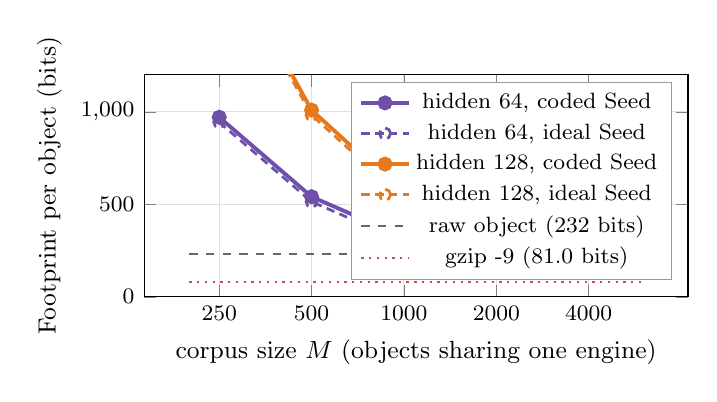
\begin{tikzpicture}
\begin{axis}[width=0.7\textwidth,height=4.4cm,xmode=log,
  xlabel={corpus size $M$ (objects sharing one engine)}, ylabel={Footprint per object (bits)},
  grid=major, grid style={black!12}, ymin=0, ymax=\figYmax,
  xtick={250,500,1000,2000,4000}, xticklabels={250,500,1000,2000,4000}, log ticks with fixed point,
  legend style={font=\footnotesize,draw=black!40,at={(0.97,0.97)},anchor=north east},
  every axis label/.style={font=\small}, tick label style={font=\footnotesize}]
  \designBPlots{}
  \addplot[black!60,dashed,thick,domain=200:6000] {232}; \addlegendentry{raw object (232 bits)}
  \addplot[cSeed,dotted,thick,domain=200:6000] {\gzipBits}; \addlegendentry{gzip -9 (\gzipBits{} bits)}
\end{axis}
\end{tikzpicture}
\caption{Amortisation curve of the predictive engine. The per-object Footprint is $|\weights|/M+|\seed|$:
the weight term vanishes as the corpus grows and the curve crosses below the raw object size
at the break-even corpus size $M^{*}=|\weights|/(N-|\seed|)$.}
\label{fig:amort}
\end{figure}

Every object, including the 200 never seen, regenerates bit-exactly. At $M=4000$ the 64-unit
engine holds 116\,KB of text in 76\,KB ($0.66\times$ raw; \texttt{gzip -9} over the whole corpus
is $0.35\times$, so this is the amortisation mechanism demonstrated, not yet a win), crossing
below the raw size at $M^{*}\approx1600$--$3200$ objects; held-out Seeds are only 3--7 bits longer than training Seeds,
so the engine learned the language, not the corpus. The Seed alone (67--94 bits ideal) is already
at or below \texttt{gzip}'s 81 bits; what keeps the total above \texttt{gzip} on this small corpus
is the weight term, which halves every time the corpus doubles.

\subsection{Whole files, and where a 148\,KB engine stands among standard compressors}
\label{sec:realfile}
The predictive engine was trained on 2\,MB of English (five books) and frozen as the shared
generator: \engineBytes{} bytes. Whole files are processed in \blockLen{}-byte blocks from the
zero state: \emph{stream} mode runs one range coder over all blocks (smallest Seed, sequential
read); \emph{blocks} mode gives every block its own stream and batches the engine across blocks
(block-parallel; Proposition~\ref{thm:law}(iv)) with a per-block \emph{verbatim escape}---a block
the engine cannot shorten is stored raw, so the Footprint never exceeds the file by more than two
bytes per block. Table~\ref{tab:realfile} stores four files as single objects.

\begin{table}[!htb]
\centering\small
\caption{Real files as single objects with the 55\,KB English engine (shared, counted once).
Write = closed-form Seed Discovery, read = Manifestation; every regenerated file matched its
sha-256. \texttt{pg12.txt} here is the raw Project Gutenberg file including its header and
licence (196,534\,B); Tables~\ref{tab:multi}--\ref{tab:n8} use the book's body alone
(176,754\,B).}
\label{tab:realfile}
{\footnotesize\setlength{\tabcolsep}{3pt}\realfileTable{}}
\end{table}

On the book the engine never saw (\texttt{pg12}, \emph{Through the Looking-Glass}) the Seed is
2.65 bits per byte, $0.33\times$: below \texttt{gzip}, 5\,\% above \texttt{xz}. The PNG exposes
both ends of the law: in stream mode the mismatched engine \emph{expands} it to $1.73\times$
(the floor made visible); in blocks mode the escape stores every block raw at $1.008\times$ (the
ceiling, implemented) and reads in 0.2\,s. Out-of-domain text sits between, and there the engine
loses to \texttt{gzip}. To test whether the loss to \texttt{xz} is a property of the approach or
of the budget, a larger engine (hidden 256, 512-byte blocks, \nEightBytes{} bytes) was trained on
12\,MB from sixteen texts (fifteen Gutenberg books and \emph{Alice}) with two books held out
entirely (Table~\ref{tab:n8}); one caveat is that \texttt{pg12}, \emph{Through the
Looking-Glass}, is the sequel to \emph{Alice} by the same author, so its style is not wholly
unseen, whereas \texttt{pg84}, \emph{Frankenstein}, has no relative in the corpus. Both come out
\emph{below} \texttt{xz -9} and \texttt{bz2 -9}, by 13\,\% and 18\,\% against \texttt{xz}, and the
fixed-point engine of Section~\ref{sec:determinism} gives up about 4\,\% of that and is still
below \texttt{xz}. These are Seed sizes: the engine is paid once and, at a 5.4\,\% saving over
\texttt{xz}, is repaid after about 2.8\,MB of unseen books---roughly ten of this size.

\begin{table}[!htb]
\centering\small
\caption{The larger English engine on two books it never saw. ``float'' is stream mode;
``fixed/C'' the integer engine in compiled blocks mode. All bit-exact.}
\label{tab:n8}
{\footnotesize\setlength{\tabcolsep}{3pt}\nEightTable{}}
\end{table}

\textbf{Beating \texttt{xz} is a low bar for text}, and Table~\ref{tab:baselines} adds the
baselines a compression reviewer would ask for, on the same bytes. PPMd \citep{cleary1984,shkarin2002}, the
classical context-model text compressor as shipped in 7-Zip, with \emph{no} training data and no
engine to store, is below the engine on both books, by \ppmdGap{}\,\% over the two; given the same
12\,MB corpus as a prior it is \ppmdPriorGap{}\,\% below. Brotli \citep{alakuijala2016brotli}, which
ships a 122\,KB static dictionary---the closest existing analogue of a shared engine---and
\texttt{zstd} with a \baselineDictBytes{}-byte dictionary trained on the engine's own corpus
\citep{collet2021zstd} both stay above the engine. The fixed-point engine, which is what a
device would carry, is beaten by \texttt{bz2} on \texttt{pg12}. The honest reading is that a
148\,KB recurrent engine is a PPM-class text compressor, not a state-of-the-art one: the residue it
leaves is about 2.1 bits per character where PPMd leaves 2.0 and cmix-class models about 1.2.
What the engine offers that PPMd does not is not ratio but the device properties the rest of the
paper measures---a fixed, shared, hash-named generator in integer arithmetic that regenerates the
same bytes on any implementation, block-parallel, selectable per object by a Manifest beside
procedural, delta and retrieval engines---and a path to lower residue through engine size, since
this engine is a thousandth of cmix's. This paper claims no compression record on text.

\begin{table}[!htb]
\centering\small
\caption{Stronger baselines on the two held-out books (ratio to raw; same byte strings as
Table~\ref{tab:n8}; bold = best without a prior). ``$+$ dict'' is \texttt{zstd --ultra -22} with
a \baselineDictBytes{}-byte dictionary trained on the engine's 12\,MB corpus; ``$\mid$ prior'' is
$|\mathrm{compress}(\mathrm{corpus}\,\|\,\mathrm{book})|-|\mathrm{compress}(\mathrm{corpus})|$, the
compressor given the engine's corpus. Reproduced by \texttt{baselines.py}.}
\label{tab:baselines}
{\scriptsize\setlength{\tabcolsep}{2.6pt}\baselineTable{}}
\end{table}


\subsection{Domain engines, revisions and libraries on one disk}
\label{sec:multi}
A production disk carries several engines and the Manifest's GID selects one per object; at write
time the disk tries every applicable engine and keeps the smallest Seed, with the escape always a
candidate. Table~\ref{tab:multi} puts four on one disk: \textbf{ANET-EN}, the English engine;
\textbf{ANET-CODE}, the same architecture trained on 2\,MB of CPython source; \textbf{ANET-LIB},
a larger engine (hidden 384) trained on one document until its surprisal there is small; and
\textbf{ANET-PROC}, a procedural engine---a Lorenz simulator \citep{lorenz1963} whose Seed is its
parameter record and whose Manifestation reruns it.

\begin{table}[!htb]
\centering\small
\caption{One disk, four engines. ``ratio'' is Seed/size with engines shared; ``total'' adds the
chosen engine's bytes, the number for a single-object disk. All bit-exact.}
\label{tab:multi}
{\scriptsize\setlength{\tabcolsep}{2.5pt}\multiTable{}}
\end{table}

The simulation output regenerates from a 118-byte record ($10^{-4}$; \texttt{xz}: 0.31). The
library engine stores its document at $0.14\times$ against 0.32 for \texttt{xz}, but is larger than
a one-document library, so the total is $1.59\times$: three more hours of training took the Seed to
$0.094\times$ and the total nowhere, because the information merely moved from Seed to weights.
Engine selection did the rest---the \emph{Frankenstein} excerpt to ANET-EN ($0.34\times$; a
favourable case, since that book is in the 55\,KB engine's training corpus, unlike in
Table~\ref{tab:n8}), Python source to ANET-CODE ($0.46\times$; \texttt{xz} 0.31), the PNG to the
escape---without being told anything about domain.

\textbf{Revisions cost their edits.} Weights never change when an object is written, so a
revision of an object already on the disk should not pay for it again. The \emph{delta engine}
makes a Seed a reference to a base object plus a token-level edit script (Ratcliff--Obershelp
matching via \texttt{difflib}, \citealp{ratcliff1988}); the disk tries a delta against every
existing text object, so lineage is discovered rather than declared. Four versions of one
document (Table~\ref{tab:edit}): a 60-word revision costs 390 bytes ($0.0022\times$), a further
revision with an appendix 390 bytes, a version with 5\,\% of all words changed 4,543 bytes;
the four together occupy 30,124 bytes of Seeds against 223,328 for \texttt{xz} on each. Counting
the engine: with the library engine the four cost 286,804 bytes, more than \texttt{xz}; with the
shared 55\,KB English engine storing the base they cost 126,136, 44\,\% below---the deltas are the
same under either.

\begin{table}[!htb]
\centering\small
\caption{Four versions of one document. Each was written with the library engine and, where
smaller, as a delta against the best existing base. All bit-exact. Read times here were measured
while a training job shared the machine's single core; Table~\ref{tab:multi} has the same
engine and object unloaded (12\,s).}
\label{tab:edit}
{\footnotesize\setlength{\tabcolsep}{2.8pt}\editTable{}}
\end{table}

\textbf{Library documents cost a reference.} Memorising a library with a neural engine is slow:
\libworkShort{} So
the \emph{retrieval engine} instead stores the library once as a content-addressed index of
content-defined chunks (gear hash after FastCDC, \citealp{xia2016fastcdc}; mean 64 bytes) and
predicts only what is not already there: a Seed is a layout of library runs interleaved with new
segments, the new bytes coded by the English engine. The index is shipped once
(\retEngineBytes{} B for a \retLibraryBytes{}-byte, two-document library). Manifestation retrieves the runs, decodes the residual and assembles. A library document
then costs 10 bytes---one run covering the whole document, regenerated in milliseconds from the
index, the $0.01\times$ mark passed by two orders of magnitude by construction rather than by
training (Table~\ref{tab:ret}); a composite manual stitched from sixty paragraphs of
two library documents plus new text, the case no other engine handles, $0.134\times$
(\texttt{xz}: 0.37); for pure edits the delta engine still wins ($0.0022\times$ against $0.020\times$), because a
changed word costs a whole chunk in a layout but only the word in an edit script; an unseen
document finds no runs and costs exactly what the English engine costs. Retrieval never hurts,
and the disk chose among four engines per object without being told anything about lineage or
domain. It is de-duplication
\citep{muthitacharoen2001,tridgell1996} fused with a predictor: the cache corner of the triangle.

\begin{figure}[!htb]
\centering
\libworkPlot{}
\caption{Footprint against training Work ($\Work_{\mathrm{train}}$): the library document's Seed ratio at twelve checkpoints of the library engine, one core. The curve flattens near $0.1\times$; the information moves from Seed to weights, and the total does not fall.}
\label{fig:libwork}
\end{figure}

\begin{table}[!htb]
\centering\small
\caption{Retrieval engine beside the library, delta and English engines; every engine tried, the
smallest Seed wins. All bit-exact. \texttt{rev3\_5pct.txt} is a fresh random 5\,\% revision
generated for this experiment, hence its size differs from Table~\ref{tab:edit}.}
\label{tab:ret}
{\footnotesize\setlength{\tabcolsep}{2.6pt}\retTable{}}
\end{table}

\subsection{Determinism: one engine, two implementations, identical bytes}
\label{sec:determinism}
A Seed is only worth storing if it regenerates the same object on every device. A float engine
cannot promise this: its probability tables depend on the order in which a dot product is
summed, which differs between BLAS libraries, core counts and GPUs, and one differing table
desynchronises the coder. The \emph{fixed-point engine} removes the dependence by construction:
Q12 integer weights, Q15 integer state, table-driven $\tanh$ and $2^{x}$, int64 accumulators,
integer soft-max---no floating point between Seed and object, obtained by post-hoc quantisation
of the trained engine \citep{jacob2018}. The harness encodes and decodes three objects under
three ways of evaluating a dot product---plain, split-and-added (a different summation order),
and float64 accumulation (a different precision)---and compares Seeds and tables against a
reference (Table~\ref{tab:determinism}). The float engine fails every cross-variant case; the
fixed-point engine passes all nine at essentially the same Footprint (10,035 against 10,046 bytes
on the text). Its products stay below $2^{40}$, so by construction any device with 64-bit integers
should yield the same bits; what has been \emph{verified} is three evaluation orders on one CPU and
two independent implementations. The engine and coder were re-implemented in C (OpenMP over
blocks): the C Seeds are byte-identical to the Python ones and each decodes the other's, so the
specification is complete; it runs ${\sim}9\times$ faster (58\,KB/s per core against 6.5),
storing 3.4\,MB of five books at 0.342 in 58\,s (Table~\ref{tab:fast}). The engine spends
${\sim}49{,}000$ multiply--adds per byte, so throughput is set by arithmetic, not by the coder; the
test machine's single physical core gives block parallelism only $1.1\times$, and Horizon against
cores needs a multi-core host.



\begin{table}[!htb]
\centering\small
\caption{Cross-arithmetic determinism, three objects (text, Python, PNG). Cells are objects
passing out of three; PASS = identical Seed and bit-exact regeneration of the reference Seed.}
\label{tab:determinism}
{\footnotesize\setlength{\tabcolsep}{4pt}\detTable{}}
\end{table}

\begin{table}[!htb]
\centering\small
\caption{Compiled fixed-point engine (hidden 128), blocks mode, by OpenMP thread count on a
machine with one physical core and two hardware threads.}
\label{tab:fast}
{\footnotesize\setlength{\tabcolsep}{4pt}\fastTable{}}
\end{table}

\subsection{Deep data at scale, and a scaling check with 1000 files}
\label{sec:deepscale}
\label{sec:proof1000}
Two objects of flight size were stored as procedural Manifests with generators written in
\emph{integer} arithmetic, bit-identical on any machine: 2.5 million records of synthetic attitude
telemetry (a Lorenz system in Q20 fixed point standing in for a rigid-body simulation, 104.6\,MB) and an $8192\times8192$ 16-bit
elevation model from hash-based integer value noise (fractal noise after \citealp{perlin1985};
SplitMix64 mixing, \citealp{steele2014splitmix}; 134.2\,MB). Both regenerate bit-exactly
(Table~\ref{tab:deepscale}): the telemetry costs 122 bytes of Seed plus 842 of program,
$9\times10^{-6}$ of its size, against 0.248 for \texttt{xz}, which also needed 170\,s to compress
it, fifteen times the 11\,s the engine needs to regenerate it. The elevation model is the harder case for a
compressor (0.552 for \texttt{xz}) and the same trivial case for the engine ($1.2\times10^{-5}$).
The disk file holding both Manifests is 895 bytes; with the two programs, 3.3\,KB for 239\,MB, a
ratio of $7\times10^{4}$ (the decoder itself, a Python interpreter, is not counted, just as the
\texttt{xz} binary is not). On a flight-class processor the telemetry regenerates in minutes and
the model in a quarter of an hour---Horizons a probe on a months-long cruise does not notice. To be explicit about what this shows:
both objects were produced by programs written for the experiment, so their Footprint is
\emph{provenance capture by construction}, not a discovery about the data. The experiment
demonstrates the mechanism, the accounting and the Horizon at scale; its value in a mission is
proportional to the share of data that is program output---all of simulation, rendering and
synthetic products, none of raw sensor data.

\begin{table}[!htb]
\centering\small
\caption{Deep data at scale (Footprint counts Seed and program; \texttt{gzip -6}/\texttt{xz -6}
because of the sizes; the flight-class column scales the measured time by ten and is indicative
only---a RAD750/LEON-class processor may be thirty times slower).}
\label{tab:deepscale}
{\footnotesize\setlength{\tabcolsep}{2.4pt}\deepTable{}}
\end{table}

\textbf{Scaling check with 1000 files.} The Conclusion's arithmetic was checked rather than
asserted: one thousand distinct synthetic-telemetry runs were stored on a disk holding only the generator program and a
catalogue of one thousand Manifests. Phase A generated each file once, recorded its length and
sha-256 and discarded it (the moment at which, in a real system, the file was written); phase B
regenerated every file from the catalogue \emph{alone} and checked the digest; phase C queried the
catalogue. \proofSection{}

\subsection{Ten files through one disk}
\label{sec:demo}
The released \texttt{demo/} folder runs the paradigm as a user would see it: ten files of
1--5\,MB (four public-domain books never used to train any engine, three PDFs, two uncompressed
procedural animations and a NASA H.264 video) are written to a disk folder holding only engines,
Seeds and Manifests, then regenerated from that folder alone and compared byte-for-byte. The disk
carries the 256-unit English engine in compiled fixed-point form, the animation engine that made
two of the videos, and the escape.

\begin{table}[!htb]
\centering\small
\caption{Ten files through one \adisk{}. ``engine$/$10'' is the shared engine (201,006\,B:
the int8 English engine plus the animation generator's source) divided by the ten files that share
it; ``Seed $+$ engine$/$10'' is what each file effectively occupies; ``output'' is the size of the
regenerated file, byte-identical to its input in every row. \texttt{xz -6} for comparison.}
\label{tab:demo}
{\scriptsize\setlength{\tabcolsep}{2.4pt}\demoTable{}}
\end{table}

Read the table as a skeptic would. Across the ten, Seeds plus engine occupy 0.494 of the input (0.495
with the Manifests) against 0.422 for \texttt{xz -6}: on this mixed set the disk \emph{loses} to a free, standard compressor,
because four files sit at $1.000\times$---a PDF of page images, a Flate-compressed PDF, an H.264
video and a PDF whose text is hex-encoded in its content streams---for which no engine on this
disk exists, so the escape keeps their bytes rather than expand them. The four unseen books, at
$0.27$--$0.29\times$, are on par with \texttt{xz}: creditable for a 148\,KB engine, but parity, not
a breakthrough. The two animations, 3.5 and 2.7\,MB stored as 110-byte parameter records, are
the only dramatic rows, and they are provenance capture: every pixel of every frame is a
deterministic function of seven numbers, the file carries about 110 bytes of information and
3.4\,MB of the program's doing, and \texttt{xz}, which looks for repeated bytes rather than for the
program, reaches only 0.446. Point a camera at the sky and record the same 3.4\,MB and no program
on any disk produces those bytes from 110 numbers---which is why the NASA video in the same table
sits at $1.000\times$. What the table demonstrates is the paradigm working end to end and the law
of Section~\ref{sec:law} visible in one place; it does not demonstrate superiority over existing
compression on general files, and this paper does not claim it. The remedy for the engine-less
files is more engines, which is a research programme rather than a result.

\subsection{What the numbers mean}
\label{sec:whynot}
\textbf{Why shared weights do not make every file cost $0.01\times$.} The Seed is the part of the
object the engine cannot predict. Shared weights remove the \emph{shared} part---for English, the
spelling, grammar and common phrases---which is why an unseen book's Seed is smaller than
\texttt{xz}. What remains is the object's own novelty: which words this author chose. That residue
is about 2.1 bits per character for the engine of Table~\ref{tab:n8}, 2.0 for PPMd, about 1.2
for cmix and NNCP on Wikipedia text ($0.15\times$), about 0.7 for a 70-billion-parameter language
model used as a coder with its size not counted \citep{deletang2023}, and Shannon put the entropy
of English near one bit per character \citep{shannon1951}, $\approx0.12\times$; $0.01\times$ is
0.08 bits per character, below the information content of the text by any of these estimates. No weights, however good or widely shared,
take a \emph{novel} object below its own information content; that is the floor, and it holds for
every storage scheme. The \emph{weight} cost per object does go to zero as objects are added
(Table~\ref{tab:designB}); the Seed cannot. So the per-object Footprint is tiny exactly when the
object is \emph{not} new to the disk: program output ($10^{-4}$--$10^{-6}$), a revision
($2\times10^{-3}$), a library document ($6\times10^{-5}$).

\textbf{Why not one engine per file.} An engine shared by nothing is part of that file's
Footprint, and engine plus Seed must then hold the file's whole information: compression by
another name, under the same floor. The single-document library engine measured it---Seed
24,801\,B, engine 256,680\,B, $1.59\times$---and further training moved information from Seed to
weights without moving the total; a network memorising bytes is a worse compressor than
\texttt{xz}, as implicit neural representations show for images. The saving comes only from
sharing: put the domain's knowledge in the engine, and every object pays only for what is
genuinely its own.

\textbf{Design rules learned.} The demo engine reached its first bit-exact object only on its
sixth revision, and the failures are rules for any \anet{}. (1)~Inject the Seed at every step
through a context-dependent projection: a Seed used only as $\mathbf{h}_0$ decays into a fixed
point (180 of 232 bits), and one injected identically at every step ties all blocks together (195
of 232). (2)~Stay out of saturation: a soft-plus loss drove 87\,\% of units into saturation,
where gradients vanish; a hinge loss with the Seed projected onto a norm ball fixed it.
(3)~Accept only \emph{quantised} Seeds that reproduce every bit with a margin. (4)~Give the
engine output feedback, or every object is a memorisation problem and the exchange rate stays
near one. (5)~Prefer closed-form discovery where it exists.

% =====================================================================
\section{The Device, Deployment and Policy}
\label{sec:device}
% =====================================================================
The \adisk{} of Section~\ref{sec:results} is a file and a program; as a device it is a sealed
unit with one input, a Manifest, and one output, the object, streamed serially and bit-exactly.
\begin{itemize}[leftmargin=1.4em,itemsep=1pt]
  \item \textbf{Input: a Regeneration Manifest}---generator identity, Seed, length, digest, block
        length, mode; a few bytes to a few kilobytes, arriving over any narrow link: a serial line,
        a radio frame, a QR code, a hand-typed string.
  \item \textbf{Output: the object, in order, as a byte stream} on a serial port, a USB endpoint,
        a socket, or directly into a consumer (a display, a printer, a guidance computer); the
        first byte is available after one engine step and the stream ends with a verified digest.
  \item \textbf{Control:} a \emph{materialise} command (write the stream to the cache), an
        \emph{evict} command, and a status line reporting the Horizon the device needs for a
        given Manifest at its Compute.
\end{itemize}

\begin{figure}[!htb]
\centering
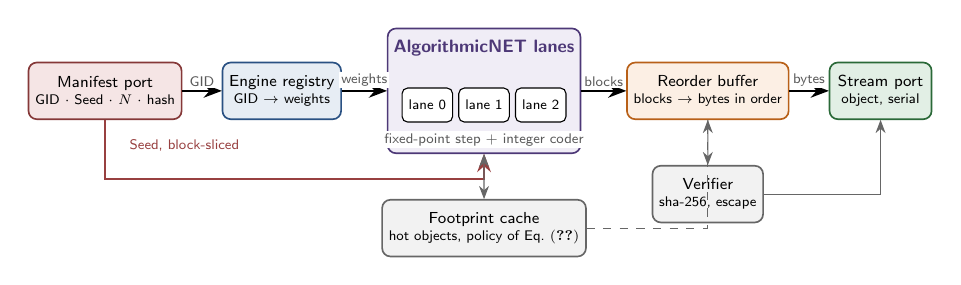
\begin{tikzpicture}[>=Stealth,font=\sffamily\small,scale=0.72,transform shape,
  box/.style={draw,rounded corners=3pt,minimum height=10mm,minimum width=18mm,align=center,line width=0.6pt,font=\sffamily\footnotesize},
  lab/.style={font=\sffamily\scriptsize,text=black!65,fill=white,inner sep=1pt}]
  \node[box,fill=cSeed!15,draw=cSeed!70!black] (in) {Manifest port\\[-1pt]{\scriptsize GID $\cdot$ Seed $\cdot$ $N$ $\cdot$ hash}};
  \node[box,fill=cFoot!12,draw=cFoot!80!black,right=7mm of in] (reg) {Engine registry\\[-1pt]{\scriptsize GID $\to$ weights}};
  \node[box,fill=cNet!10,draw=cNet!70!black,right=8mm of reg,minimum width=34mm,minimum height=22mm] (eng) {};
  \node[font=\sffamily\bfseries\small,text=cNet!70!black] at ($(eng.north)+(0,-3.5mm)$) {AlgorithmicNET lanes};
  \foreach \i in {0,1,2} \node[draw,fill=white,rounded corners=2pt,minimum width=8mm,minimum height=6mm,font=\sffamily\scriptsize] at ($(eng.center)+(-10mm+10mm*\i,-2.5mm)$) {lane \i};
  \node[lab] at ($(eng.south)+(0,2.5mm)$) {fixed-point step $+$ integer coder};
  \node[box,fill=cComp!12,draw=cComp!80!black,right=8mm of eng] (rob) {Reorder buffer\\[-1pt]{\scriptsize blocks $\to$ bytes in order}};
  \node[box,fill=cHori!15,draw=cHori!70!black,right=7mm of rob] (out) {Stream port\\[-1pt]{\scriptsize object, serial}};
  \node[box,fill=black!5,draw=black!60,below=8mm of eng,minimum width=34mm] (cache) {Footprint cache\\[-1pt]{\scriptsize hot objects, policy of Eq.~\eqref{eq:policy}}};
  \node[box,fill=black!5,draw=black!60,below=8mm of rob] (ver) {Verifier\\[-1pt]{\scriptsize sha-256, escape}};
  \draw[->,thick] (in) -- (reg) node[midway,lab,above=1pt] {GID};
  \draw[->,thick] (reg) -- (eng) node[midway,lab,above=1pt] {weights};
  \draw[->,thick] (eng) -- (rob) node[midway,lab,above=1pt] {blocks};
  \draw[->,thick] (rob) -- (out) node[midway,lab,above=1pt] {bytes};
  \draw[->,thick,cSeed!80!black] (in.south) |- ($(eng.south)+(0,-4.5mm)$) -| (eng.south) ;
  \node[lab,text=cSeed!80!black] at ($(in.south)+(14mm,-4.5mm)$) {Seed, block-sliced};
  \draw[->,black!60] (rob) -- (ver);
  \draw[->,black!60] (ver) -| (out);
  \draw[<->,black!60] (cache) -- (eng);
  \draw[->,black!60,dashed] (cache.east) -| (rob.south);
\end{tikzpicture}
\caption{The Regeneration Appliance. A Manifest enters; the registry selects the engine by
GID; the Seed is sliced into block streams and fed to $p$ identical fixed-point lanes; a
reorder buffer restores object order; the verifier checks the digest; the object leaves as a
serial byte stream. The cache holds materialised objects under the regenerate-versus-cache
policy.}
\label{fig:device}
\end{figure}

\textbf{Engine registry}: non-volatile memory with one integer weight set per generator identity
(55--257\,KB per engine here), so a registry of domain engines is a few megabytes of flash and
every appliance regenerates the same bytes from the same Manifest. \textbf{Lanes}: $p$ copies of
the fixed-point step and integer coder, each owning one block from $\mathbf{h}=\mathbf{0}$ with its
block code and slice of the Seed; no floating point, 4\,KB of state. \textbf{Slicer and reorder
buffer}: block $j$ goes to lane $j\bmod p$ and a $p\times L$-byte buffer releases bytes in object
order. \textbf{Verifier and escape}: the digest is checked as the stream leaves; verbatim blocks
bypass the lanes. \textbf{Cache}: optional RAM or flash under the policy below. Procedural and
delta engines are lane programs. The lane cost is fixed by the engine (${\sim}5\times10^{4}$
multiply--adds per byte for the 128-unit engine), so the appliance's Horizon is arithmetic
(Table~\ref{tab:device}); the rows are the triangle in hardware---same Manifest, same bytes, a
Horizon that shrinks as Compute is added. The appliance's Footprint is its registry plus its
Manifests---every engine of this paper and a million Manifests is a few hundred megabytes---while
its apparent capacity is the sum of the objects they regenerate.

\begin{table}[!htb]
\centering\small
\caption{Streaming rate against Compute, 128-unit engine. Only the first row is measured; the
others are illustrative upper bounds from the multiply--add count and assume the lanes are kept
busy, which a sequential recurrence does not guarantee on wide hardware.}
\label{tab:device}
\begin{tabular}{@{}lllrr@{}}
\toprule
realisation & Compute & lanes & rate & 100\,MB object \\
\midrule
this paper, one x86 core, C & ${\sim}3\,$GMAC/s eff. & 1--2 & 58\,KB/s (meas.) & 29\,min \\
microcontroller (Cortex-M7 class) & 0.2\,GMAC/s (est.) & 1 & 4\,KB/s & 7\,h \\
FPGA, 64 DSP lanes at 200\,MHz & 13\,GMAC/s (est.) & 64 & 250\,KB/s & 7\,min \\
GPU module (int8, $10^{4}$ lanes) & 10\,TMAC/s nominal & $10^{4}$ & $\le$200\,MB/s & $\ge$0.5\,s \\
\bottomrule
\end{tabular}
\end{table}

\textbf{Where the trade pays, and where it does not.} On Earth a byte at rest is nearly free:
flash costs of the order of a cent per gigabyte, and a microSD card holds more than every object
in this paper. Regenerating a file over hours to save such bytes is never worth it, and the
paper does not propose it. The trade pays where the scarce quantity is not the byte at rest but
the byte \emph{in transit} over a narrow link (a deep-space uplink of kilobits per second, a text
message), the byte that must \emph{survive} a medium or a lifetime that flash cannot, or the
verification that what arrived is exactly what was sent; the Manifest is the unit of all three.
The regimes below are chosen on that criterion.

\textbf{Deployments} (Table~\ref{tab:deploy}). An interplanetary probe pays in Horizon:
manuals, maps and model updates regenerated over months of cruise from Manifests of a few
hundred bytes, uplinked from a ground segment that keeps the same registry and discovers Seeds
with data-centre Compute. A solar outpost regenerates on demand, deletes what is idle and recreates
it later, using sunlight as storage. A millennial archive keeps centuries of records in a small
vault, accepts hours per retrieval, and is queried through its catalogue of Manifests without
regenerating anything. A school without internet has the shape of a probe---a narrow, intermittent link (a phone with
SMS, a community radio, a USB stick carried by a visitor) and patient users. The appliance is a
single-board computer or a solar laptop carrying the engine registry and a catalogue in which
every textbook, lecture and dataset is a Manifest of a few hundred bytes to a few kilobytes, so a
whole curriculum's catalogue fits in a feature phone's memory; the value is the link, not the
storage it saves. A revised chapter is its edits alone and a new title a Seed against the engines
already on site, so a term's updates arrive in one text message or one radio pass. Content is
created on demand from the \anet{} and the Seeds: a teacher deletes last month's chapter to make
room for the next one, starts its regeneration the day before while the panel charges, and finds
it in the cache for class; the deleted chapter loses only its bytes and returns from its Seed when
needed; and the digest in every Manifest tells the teacher that what the students read is exactly
what was sent. A remote spacecraft is the same design at a greater distance: it restores whatever
it needs from the condensed source it carries---engines, Seeds, Manifests---and discards the bytes
when done. For
deep space the lane array is a radiation-tolerant FPGA, the registry lives in flight flash, and
the ground, because the engine is fixed-point, verifies before uplink the exact bytes the probe
will produce. The data centre is where Seed Discovery for all of the above is done.

\begin{table}[!htb]
\centering\small
\caption{Operating points on the Regeneration Triangle (``$\uparrow$'' abundant, ``$\downarrow$'' scarce).}
\label{tab:deploy}
\begin{tabular}{@{}lccclp{4.5cm}@{}}
\toprule
\textbf{Deployment} & $\Foot$ & $\Comp$ & $\Hori$ & \textbf{Pays with} & \textbf{Example} \\
\midrule
Interplanetary probe & $\downarrow$ & $\downarrow$ & $\uparrow\uparrow$ & Horizon & manuals, maps, models regenerated over months of cruise \\
Planetary outpost & $\downarrow$ & $\uparrow$ (solar) & $\uparrow$ & Compute $\times$ Horizon & regenerate on demand, delete when idle, recreate later \\
Millennial archive & $\downarrow\downarrow$ & $\downarrow$ & $\uparrow\uparrow\uparrow$ & Horizon & centuries of records in a small vault; hours per retrieval \\
Palm-scale device & $\downarrow$ & $\downarrow$ & medium & amortised weights & one shared engine, thousands of Seeds \\
Off-grid school & $\downarrow$ & medium & $\uparrow$ & Horizon $+$ engines & one solar board holds a whole library as Manifests \\
Data centre & $\uparrow$ & $\uparrow\uparrow$ & $\downarrow$ & Compute & Seed Discovery for all of the above \\
\bottomrule
\end{tabular}
\end{table}

\textbf{Regenerate-versus-cache policy.} Space is bought once; time is paid on every read. A
stored byte costs its space for as long as it exists, whereas a regenerated object costs its
Horizon each time it is read, so the space-for-time conversion is a rental rather than a purchase.
With $c_{\Foot}$ the cost per byte-second of storage and $c_{\Work}$ the cost per operation, an
object accessed $\lambda$ times per second should be cached iff
\begin{equation}
  \lambda>\lambda^{*}=\frac{c_{\Foot}\,N}{c_{\Work}\,\Work_{\mathrm{read}}(N)},
  \label{eq:policy}
\end{equation}
the rate at which the device decides, object by object, whether to rent time or buy space. On a
solar-powered node $c_{\Work}$ falls to nearly zero in daylight, driving $\lambda^{*}$ up and the
resident cache down: the system uses sunlight as storage. Eq.~\eqref{eq:policy} is the design
rule for experiment E4 and has not yet been measured.

% =====================================================================
\section{Open Experiments and Future Work}
\label{sec:future}
% =====================================================================
The experimental programme and its status are in Table~\ref{tab:programme}; a GPU run of the
determinism harness is the sixth open item.

\begin{table}[!htb]
\centering\small
\caption{Experimental programme. Each measures one exchange rate of the triangle.}
\label{tab:programme}
\begin{tabular}{@{}llp{4.8cm}p{2.8cm}p{3.4cm}@{}}
\toprule
\textbf{Exp.} & \textbf{Name} & \textbf{Measures} & \textbf{Data} & \textbf{Status} \\
\midrule
E1 & Frontier sweep & $\Foot^{*}(\Work)$ per data class under increasing Work budgets & simulation, telemetry, images, text, random & planned \\
E2 & Seed Discovery & Footprint vs.\ write-time Work for the discovery strategies & 232-bit object; procedural data & Table~\ref{tab:sweep} (miniature) \\
E3 & Amortisation & per-object Footprint vs.\ corpus size $M$ with a shared engine & Alice corpus; whole books & Tables~\ref{tab:designB}--\ref{tab:ret} \\
E4 & Policy & realised cost of Eq.~\eqref{eq:policy} on a solar power trace & outpost workload replay & planned \\
E5 & Substitution & Horizon vs.\ cores for block-parallel manifestation & a 1\,TB object & compiled coder built; needs a multi-core host \\
\bottomrule
\end{tabular}
\end{table} \noindent\textbf{Hypotheses and status.} (H1) On deep data $\Foot^{*}(\Work)$ falls by orders of
magnitude at modest Work---\emph{supported} (Tables~\ref{tab:multi} and~\ref{tab:deepscale}).
(H2) Amortised per-object Footprint decreases monotonically with $M$---\emph{confirmed}
(Table~\ref{tab:designB}). (H3) Manifestation Horizon scales as $1/p$ in the number of cores
$p$---\emph{not yet testable} on a single-core machine. (H4) The policy of Eq.~\eqref{eq:policy}
reduces resident Footprint by $\ge90\,\%$ on an outpost replay at no loss of
availability---\emph{planned}.

\textbf{Parallel manifestation.} Within a block every engine here emits
its bits in series, and serial emission is what makes Horizon the price of Footprint. Three
layouts are proposed. \emph{Segment} parallelism, the blocks mode already built, costs a few
percent of Seed and one flush per segment. \emph{Interleaved} (strided) parallelism has lane $\ell$ of $p$
emit bits $\ell,\ell{+}p,\ell{+}2p,\dots$, so each step across the lanes is one contiguous word
of the object, streamed in order with no reassembly; the lanes share the Seed injection and the
block code, and for a predictive engine the open question is making them conditionally
independent given the shared state, by a bit-plane or residue-class factorisation of the
next-symbol distribution. \emph{Hierarchical} parallelism has
a coarse engine emit a sketch and fine engines fill the gaps in parallel; the serial path would
shrink from $N$ to $O(N/2^{k}+k)$ if the fine engines can be conditioned on sketch points without
loss, an untested assumption. In every layout only the order of emission changes---the practical
form of Proposition~\ref{thm:law}(iv).

% =====================================================================
\section{Related Work and Attribution}
\label{sec:related}
% =====================================================================
The backbone is Kolmogorov complexity, its resource-bounded variants and Bennett's logical depth;
cryptanalytic time--memory trade-offs \citep{hellman1980} are the classical template for an
exchange law between storage and computation, and the triangle adds time as a separately budgeted
side and applies the trade to data at rest. ``Algorithmic networks'' \citep{abrahao2017} is an
unrelated construct; the name \anet{} is not derived from it. As a coder the predictive engine is
the classical model-plus-entropy-coder construction \citep{witten1987,martin1979}, of which PPM
\citep{cleary1984,shkarin2002} is the context-model form that Table~\ref{tab:baselines} shows
still beats the engine, and cmix \citep{knoll2014cmix}, NNCP \citep{bellard2019nncp} and
\citet{deletang2023} the neural form, reaching 1.2 bits per byte and below with models thousands
of times larger than the 55--148\,KB engines here; shared static or trained dictionaries
\citep{alakuijala2016brotli,collet2021zstd} are the existing form of a prior amortised across
objects; integer-only networks for cross-platform deterministic entropy coding were introduced
by \citet{balle2019integer}, and the fixed-point engine of Section~\ref{sec:determinism} applies
the same principle to a recurrent byte predictor; this paper does not compete with them on ratio but uses the construction as one
engine among several inside a storage device, adding the Manifest, engine selection, the escape,
the determinism guarantee and the deployment model, and measuring the trade the device makes
rather than the compression a model achieves. Implicit neural representations
\citep{dupont2021coin,sitzmann2020siren,mildenhall2020nerf} and auto-decoders
\citep{park2019deepsdf} are the relatives of the latent-Seed design; content-defined chunking
\citep{muthitacharoen2001,xia2016fastcdc} and delta transfer \citep{tridgell1996} are the ancestors
of the retrieval and delta engines; rematerialisation \citep{chen2016checkpoint} is the same trade
inside one training run; integer-only inference \citep{jacob2018} is used here for the property \citet{balle2019integer}
identified, identical output across devices. The seed-driven, inverse-manifestation view is shared
with the EmbryonicAL model \citep{patil2026embryonical}: it grows a \emph{model} from a Seed; the
\anet{} grows \emph{data}. Landauer's principle \citep{landauer1961} bounds the energy side of
Compute; reversible computing \citep{bennett1973} suggests the energy cost of manifestation, unlike
its Footprint, has no floor. Nothing in the implementation's building blocks is claimed as new:
Subbotin's carry-less range coder, FastCDC's gear hash, Ratcliff--Obershelp matching, teacher
forcing, the straight-through estimator, Adam, the Lorenz system, fractal value noise, SplitMix64,
NumPy \citep{harris2020numpy} and Project Gutenberg \citep{gutenberg} are all credited where used.

% =====================================================================
\section{Limitations and Final Notes}
% =====================================================================
The evidence is narrower than the vision. The engines are small and the text engines know only
English, and on novel text they sit among the standard compressors rather than above them
(Table~\ref{tab:baselines}); the deep-data objects were generated by programs written for the experiment, so those
ratios demonstrate provenance capture rather than a property of mission data; determinism has
been verified across arithmetic variants on one CPU, not yet on a GPU; Horizon against cores could
not be measured on a single-core machine; the caching policy is unmeasured. Two structural limits
matter more than any number. First, a Manifest is worthless without its engine: the disk
concentrates a whole library's survival in a few hundred kilobytes of weights that must be
preserved, replicated and kept executable---a single point of failure raw files do not have, and
the first thing an archive design must address. Second, the information floor: for novel data the
paradigm buys modest compression at large computational cost; only data predictable given what the
disk already holds buys orders of magnitude. What remains---the GPU run, Horizon against cores, the
emission schedules, the policy on a real power trace---needs only hardware this study did not
have; the released code lets anyone run them and check every result here.

\noindent\textbf{Code and test cases:} \url{https://github.com/syncaissa}.

% =====================================================================
\section{Conclusion}
% =====================================================================
Storage has always been paid for in bytes. This paper measures how far it can be paid for in
computation and time instead, under a law with a floor: an object's Footprint can fall to what
the disk cannot already predict, and no further. An \adisk{} holds engines and Seeds rather
than files: the engine's parameters are shared by every object, so an object costs its own
Seed plus an ever-smaller fraction of the engine as more objects are stored with different
Seeds---the more, the better. One unseen book costs the 148\,KB engine plus a 48\,KB Seed,
more than \texttt{xz}; a thousand cost 48.5\,KB each, 13\,\% less than \texttt{xz} and 8\,\% more
than PPMd needs with no engine at all---the engine is PPM-class, and the paper claims no
compression record. A thousand
105\,MB program-generated telemetry files---104\,GB---were stored in 317\,KB and every one
regenerated bit-exactly: provenance capture, which is what the paradigm is for, not compression
of arbitrary data. Every object regenerates bit-exactly on any device; revisions cost their edits;
239\,MB of simulation output came from 3.3\,KB. The gains are real exactly where the object has
structure an engine can hold---computational for deep data, statistical for a domain, shared
content for a library---and the exchange rate is the engine's knowledge of that structure. That is
the practical content of Proposition~\ref{thm:law}, and it is why a device that stores Seeds instead
of files is not a compression trick but a different place to stand on the Regeneration Triangle.

{\scriptsize\setlength{\bibsep}{0.4pt}\setlength{\columnsep}{12pt}
\begin{multicols}{2}\raggedright
\bibliographystyle{apalike}
\bibliography{refs}
\end{multicols}}

\vspace{6pt}
\begin{center}\small Syncaissa Systems Inc. \quad$\bullet$\quad \texttt{syncaissa@outlook.com}\end{center}
\end{document}
